\documentclass[11pt]{article}

\usepackage[letterpaper,margin=0.88in,headheight=22pt]{geometry}
\usepackage{fontspec}
\IfFontExistsTF{Charis SIL}{\setmainfont{Charis SIL}}{\setmainfont{TeX Gyre Pagella}}
\IfFontExistsTF{Arimo}{\setsansfont{Arimo}}{\setsansfont{TeX Gyre Heros}}
\usepackage{microtype}
\usepackage{amsmath,amssymb}
\usepackage{siunitx}
\usepackage{booktabs}
\usepackage{tabularx}
\usepackage{longtable}
\usepackage{array}
\usepackage{enumitem}
\usepackage{xcolor}
\usepackage{colortbl}
\usepackage{graphicx}
\usepackage{tikz}
\usetikzlibrary{arrows.meta,positioning,calc,decorations.pathreplacing}
\usepackage[most]{tcolorbox}
\usepackage{titlesec}
\usepackage{fancyhdr}
\usepackage{caption}
\usepackage{float}
\usepackage[hidelinks]{hyperref}
\usepackage{lastpage}
\usepackage{needspace}
\usepackage{graphbox} % Extends graphicx

% University of Texas at Austin brand palette
\definecolor{UTBurntOrange}{HTML}{BF5700}
\definecolor{UTCharcoal}{HTML}{333F48}
\definecolor{UTLightOrange}{HTML}{F8971F}
\definecolor{UTWarmGray}{HTML}{D6D2C4}
\definecolor{UTSlate}{HTML}{9CADB7}
\definecolor{UTBlue}{HTML}{005F86}
\definecolor{UTBlueBright}{HTML}{00A9B7}
\definecolor{UTWarmLight}{HTML}{F6F5F2}
\definecolor{UTBlueLight}{HTML}{EEF5F7}
\definecolor{UTGrayLight}{HTML}{F4F5F6}

% Backward-compatible semantic aliases used throughout the document
\colorlet{Navy}{UTCharcoal}
\colorlet{Teal}{UTBurntOrange}
\colorlet{LightTeal}{UTBlueLight}
\colorlet{LightBlue}{UTWarmLight}
\colorlet{LightGray}{UTGrayLight}
\colorlet{MidGray}{UTCharcoal!78}
\colorlet{RuleGray}{UTWarmGray}
\colorlet{Warn}{UTLightOrange}
\colorlet{LightWarn}{UTWarmLight}

\hypersetup{
  colorlinks=true,
  linkcolor=UTBurntOrange,
  urlcolor=UTBlue,
  citecolor=UTCharcoal,
  pdftitle={Experimental Plan for Initial Characterization of the Prop-30 Glycol Salt Twin Natural Circulation Loop (STNCL)},
  pdfauthor={TRIDENT Collaboration (UT Austin, ACU, VCU)}
}

\sisetup{
  detect-all,
  per-mode=symbol,
  range-phrase=--,
  range-units=single,
  group-separator={,},
  group-minimum-digits=4,
  group-digits=integer
}

\setlength{\parindent}{0pt}
\setlength{\parskip}{5.5pt}
\setlength{\emergencystretch}{1.5em}
\setlist[itemize]{leftmargin=1.35em,itemsep=2.5pt,topsep=3pt}
\setlist[enumerate]{leftmargin=1.55em,itemsep=3pt,topsep=3pt}
\renewcommand{\arraystretch}{1.18}
\titlespacing{\paragraph}{0pt}{0.5ex plus 0.5ex minus .2ex}{1em}

\titleformat{\section}
  {\Large\sffamily\bfseries\color{UTBurntOrange}}
  {\thesection}{0.65em}{}
  [\vspace{1pt}\color{UTWarmGray}\titlerule]
\titleformat{\subsection}
  {\large\sffamily\bfseries\color{UTCharcoal}}
  {\thesubsection}{0.6em}{}
\titleformat{\subsubsection}
  {\normalsize\sffamily\bfseries\color{UTCharcoal}}
  {\thesubsubsection}{0.55em}{}
\titlespacing*{\section}{0pt}{14pt}{7pt}
\titlespacing*{\subsection}{0pt}{11pt}{4pt}
\titlespacing*{\subsubsection}{0pt}{8pt}{2pt}

% Keep a heading from being stranded alone at the bottom of a page:
% require room for the title plus a few body lines, else break to the next page.
\usepackage{etoolbox}
\pretocmd{\section}{\needspace{5\baselineskip}}{}{}
\pretocmd{\subsection}{\needspace{7\baselineskip}}{}{}
\pretocmd{\subsubsection}{\needspace{5\baselineskip}}{}{}

\pagestyle{fancy}
\fancyhf{}
\fancyhead[L]{\small\sffamily\color{UTCharcoal}Prop-30 Glycol STNCL \textbullet\ TRIDENT}
\fancyhead[R]{\small\sffamily\color{UTBurntOrange}Experimental Plan -- Draft}
\fancyfoot[L]{\small\sffamily\color{UTCharcoal!78}Revision 0.2}
\fancyfoot[R]{\small\sffamily\color{UTCharcoal!78}Page \thepage\ of \pageref{LastPage}}
\renewcommand{\headrulewidth}{0.65pt}
\renewcommand{\headrule}{\hbox to\headwidth{\color{UTBurntOrange}\leaders\hrule height \headrulewidth\hfill}}
\renewcommand{\footrulewidth}{0pt}

\newtcolorbox{recommendbox}[1][]{
  enhanced,
  breakable,
  colback=UTWarmLight,
  colframe=UTBurntOrange,
  colbacktitle=UTBurntOrange,
  boxrule=0.7pt,
  arc=1.2mm,
  left=3mm,right=3mm,top=2.4mm,bottom=2.4mm,
  title={#1},
  fonttitle=\sffamily\bfseries,
  coltitle=white
}

\newcommand{\Tavg}{T_{\mathrm{avg},4}}
\newcommand{\Tdiag}{T_{\mathrm{diag}}}
\newcommand{\Thot}{T_{\mathrm{hot}}}
\newcommand{\Tcold}{T_{\mathrm{cold}}}
\newcommand{\QHs}{\dot Q_{H}^{s}}
\newcommand{\QCs}{\dot Q_{C}^{s}}
\newcommand{\mdotp}{\dot m_{p}}
\newcommand{\mdotpH}{\dot m_{p,H}}
\newcommand{\mdotpC}{\dot m_{p,C}}
\newcommand{\Tamb}{T_{\mathrm{amb}}}
\newcommand{\Rey}{\mathrm{Re}}
\newcommand{\Realpart}[1]{\Re\left(#1\right)}

\begin{document}
\hypersetup{pageanchor=false}

% -----------------------------------------------------------------------------
% Title page
% -----------------------------------------------------------------------------
\begin{titlepage}
\thispagestyle{empty}

\begin{tikzpicture}[remember picture,overlay]
  \fill[UTBurntOrange] (current page.north west) rectangle ([yshift=-0.16in]current page.north east);
  \fill[UTWarmLight] ([yshift=1.45in]current page.south west) rectangle (current page.south east);
  \fill[UTBurntOrange] (current page.south west) rectangle ([yshift=0.16in]current page.south east);
\end{tikzpicture}

\vspace*{-0.75in}
\noindent\includegraphics[width=2.5in]{images/TRIDENT_logo.png}

%\vspace{0.20in}
{\color{UTWarmGray}\rule{\textwidth}{0.8pt}}
\vspace{0.24in}

\begin{tcolorbox}[
  enhanced,
  frame hidden,
  colback=white,
  boxrule=0pt,
  borderline west={4pt}{0pt}{UTBurntOrange},
  left=5mm,right=0mm,top=1mm,bottom=1mm,
  sharp corners
]
{\raggedright\sffamily\bfseries\fontsize{25}{29}\selectfont\color{UTCharcoal}
Experimental Plan for the Initial Characterization of the Prop-30 Glycol Salt Twin Natural Circulation Loop (STNCL)\par}
\vspace{0.13in}
{\sffamily\fontsize{12.5}{16}\selectfont\color{UTBurntOrange}
Heat-loss characterization, inferred natural-circulation flow, and an initial operating state matrix\par}
\end{tcolorbox}

\vspace{0.34in}

\begin{tcolorbox}[
  enhanced,
  colback=UTWarmLight,
  colframe=UTWarmGray,
  boxrule=0.6pt,
  arc=1.2mm,
  left=3.5mm,right=3.5mm,top=3mm,bottom=3mm
]
{\setlength{\parskip}{0pt}\renewcommand{\arraystretch}{1.28}
\begin{tabularx}{\textwidth}{@{}>{\sffamily\bfseries\color{UTBurntOrange}}l>{\raggedright\arraybackslash}X@{}}
Status: & Draft for team review and facility-specific completion \\
Revision: & 0.1 \\
Date: & August 1, 2026 \\
Prepared for: & TRIDENT collaboration \\
\end{tabularx}}
\end{tcolorbox}

\vfill
    \nopagebreak
    \noindent
    \includegraphics[height=2.5cm, align=c]{images/ACU.png}\hfill
    \includegraphics[height=1.5cm, align=c]{images/UT.png}\hfill
    \includegraphics[height=1.25cm, align=c]{images/VCU.png}
\vspace{-0.6in}
\end{titlepage}
\clearpage
\hypersetup{pageanchor=true}

% -----------------------------------------------------------------------------
% Front matter
% -----------------------------------------------------------------------------
\pagenumbering{roman}

\section*{Revision History}
\addcontentsline{toc}{section}{Revision History}
\begin{tabularx}{\textwidth}{@{}p{0.75in}p{1.2in}>{\raggedright\arraybackslash}X>{\raggedright\arraybackslash}p{1.15in}@{}}
\toprule
\textbf{Revision} & \textbf{Date} & \textbf{Description} & \textbf{Status} \\
\midrule

0.1 & 2026-08-02 & Initial reorganized draft for team review. & Draft \\
\bottomrule
\end{tabularx}

\vspace{0.25in}

\section*{Approval and Configuration Record}
\addcontentsline{toc}{section}{Approval and Configuration Record}
\begin{tabularx}{\textwidth}{@{}p{1.55in}X p{1.25in}p{1.05in}@{}}
\toprule
\textbf{Role} & \textbf{Signature} & \textbf{Date} & \textbf{Revision} \\
\midrule
Lead, UT & & & \\
Lead, VCU & & & \\
Lead, ACU & & & \\
\bottomrule
\end{tabularx}

\clearpage
\tableofcontents
\clearpage
\pagenumbering{arabic}

% -----------------------------------------------------------------------------
\clearpage
\section{Introduction}

\subsection{Purpose}
The purpose of this document is to define a phased experimental campaign for obtaining a small, high-quality data set that characterizes the Prop-30 glycol Salt Twin Natural Circulation Loop (STNCL) before a more comprehensive experimental plan is designed. This work is conducted under the \hbox{TRIDENT} (Thermal-fluid Research and Irradiation Digital Engineering Network Testbed) collaboration, a joint effort of the University of Texas at Austin, Abilene Christian University, and Virginia Commonwealth University. The campaign first establishes the installed measurement performance and the facility thermal boundary condition, then uses the resulting thermal model and secondary-side energy balances to characterize natural-circulation behavior and select an initial operating matrix.

The plan addresses two complementary needs:

\begin{enumerate}
    \item quantify whole-loop and distributed environmental heat gain and heat loss so that system-code mesh cells and CFD surface regions can reproduce the facility thermal boundary condition; and
    \item characterize the loop's initial operating behavior, including its demonstrated feasible region, time to reach steady state, inferred natural-circulation flow regime, and possible dependence on the path used to reach a state.
\end{enumerate}

The campaign is intentionally phased. Ambient-equilibrium and near-isothermal tests are used first to evaluate the instrumentation and calibrate the distributed heat-transfer model. Corrected heater- and cooler-side energy balances are then used to infer primary-loop mass flow and Reynolds number. Finally, a five-state cross matrix is executed to sample the effects of heater duty and mean fluid temperature over the widest practical Reynolds-number range.

% -----------------------------------------------------------------------------
\subsection{Objectives}
\label{sec:objectives}

This campaign has four objectives:

\begin{enumerate}
    \item verify the installed performance, synchronization, and consistency of the temperature, secondary-flow, thermal-duty, control, and environmental measurements;
    \item estimate whole-loop and distributed environmental heat exchange above and below room temperature, with sufficient fidelity to support system-code and CFD boundary-condition models;
    \item infer primary natural-circulation mass flow, Reynolds number, and their uncertainties from corrected heater- and cooler-side energy balances; and
    \item define a preliminary demonstrated feasible region and execute a five-state cross matrix that characterizes temperature, heater-duty, flow-regime, transition-time, and path-dependence effects.
\end{enumerate}


% -----------------------------------------------------------------------------
\subsection{Experimental Apparatus}
\label{sec:functional}

The STNCL apparatus is a closed natural-circulation glycol loop containing a heater and cooler. Primary flow is generated by buoyancy and hydraulic resistance. Figure~\ref{fig:schematic} shows the loop layout and thermocouple numbering. The heater occupies the lower diagonal section and the cooler the upper diagonal section; the two vertical legs are the cold leg on the left and the hot leg on the right. Each internal thermocouple location also has a co-located Luna fiber-optic temperature measurement. The heater and cooler sections are inclined about \SI{10}{\degree} to favor the nominal buoyancy-driven circulation direction. 

\begin{table}[H]
\centering
\caption{Measurement channels and their primary uses.}
\label{tab:channels}
{\small\renewcommand{\arraystretch}{1.13}
\begin{tabularx}{\textwidth}{@{}>{\raggedright\arraybackslash}p{1.30in}>{\centering\arraybackslash}p{0.72in}>{\raggedright\arraybackslash}X>{\raggedright\arraybackslash}X@{}}
\toprule
\textbf{Measurement} & \textbf{Quantity} & \textbf{Primary use} & \textbf{Status / limitation} \\
\midrule
Internal calibrated TCs & 4 & Fluid temperature at heater inlet, heater outlet, cooler inlet, and cooler outlet & Primary fluid-temperature measurements; calibrated previously in a five-temperature common bath \\
Luna fiber-optic temperature & 4 & Co-located temperature at the four internal stations & Independent comparison, redundancy, and transient-response information \\
Pipe-wall TCs & 12 & Pipe outside-wall temperature under insulation & Distributed thermal-model calibration; not a direct heat-flux measurement \\
Heater secondary TCs & Inlet/outlet pair & Secondary-side enthalpy change & Exact measurement locations must bound the heater closely \\
Cooler secondary TCs & Inlet/outlet pair & Secondary-side enthalpy change & Exact measurement locations must bound the cooler closely \\
Secondary mass flow & Heater and cooler & Heater and cooler thermal duty & Flow-meter calibration and fluid properties required \\
Room environment & 2 stations & Air temperature and relative humidity & Used for ambient gradients, dew point, and condensation classification \\
Outer-surface temperature & 1--2 locations & Insulation-jacket or exposed-fitting temperature near the coldest locations & Required for defensible dew-point classification; under-insulation wall TCs are not outer-surface measurements \\
Primary control and status signals & Required & Heater/cooler commands, setpoints, on/off state, controller output, valve/bypass state, cycling, alarms, and operator changes & Synchronized logging is mandatory for every run \\
\bottomrule
\end{tabularx}}
\end{table}


\begin{figure}[H]
\centering
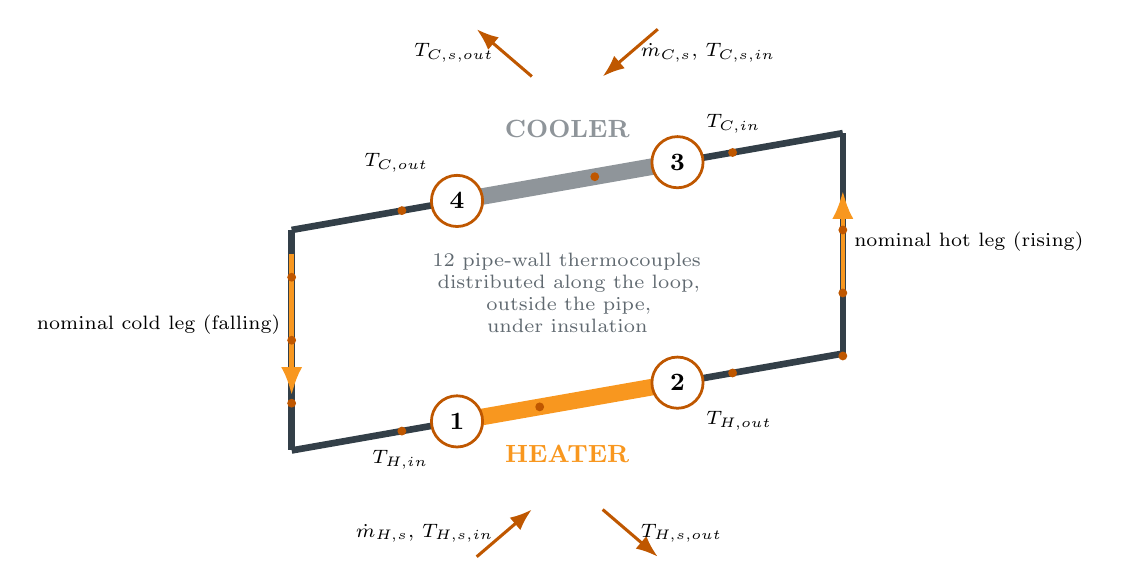
\begin{tikzpicture}[
  x=1cm,y=1cm,
  pipe/.style={line width=2.4pt,draw=Navy},
  heat/.style={line width=6pt,draw=Warn},
  cool/.style={line width=6pt,draw=Navy!55!white},
  sensor/.style={circle,draw=Teal,fill=white,line width=1pt,minimum size=6.5mm,font=\small\bfseries},
  secondary/.style={-Latex,draw=Teal,line width=1.1pt},
  flow/.style={-Latex,draw=Warn,line width=1.6pt}
]
  % corner coordinates: vertical legs at x=0 (cold) and x=7 (hot); heater/cooler diagonals at ~10 deg
  \coordinate (BL) at (0,0.6);
  \coordinate (BR) at (7,1.83);
  \coordinate (TR) at (7,4.63);
  \coordinate (TL) at (0,3.4);


  \coordinate (TOne)   at ($(BL)!0.30!(BR)$); % heater inlet
  \coordinate (TTwo)   at ($(BL)!0.70!(BR)$); % heater outlet
  \coordinate (TThree) at ($(TR)!0.30!(TL)$); % cooler inlet
  \coordinate (TFour)  at ($(TR)!0.70!(TL)$); % cooler outlet

  % pipe legs
  \draw[pipe] (TL) -- (BL); % cold leg (left, vertical)
  \draw[pipe] (BR) -- (TR); % hot leg  (right, vertical)
  % heater (lower diagonal) and cooler (upper diagonal)
  \draw[pipe] (BL) -- (BR);
  \draw[pipe] (TR) -- (TL);
  \draw[heat] (TOne) -- (TTwo);
  \draw[cool] (TThree) -- (TFour);
  \node[font=\small\bfseries,text=Warn] at (3.5,0.55) {HEATER};
  \node[font=\small\bfseries,text=Navy!55!white] at (3.5,4.68) {COOLER};

  % station sensors at the active-section boundaries
  \node[sensor,label=below left:{\scriptsize $T_{H,in}$}] at (TOne) {1};
  \node[sensor,label=below right:{\scriptsize $T_{H,out}$}] at (TTwo) {2};
  \node[sensor,label=above right:{\scriptsize $T_{C,in}$}] at (TThree) {3};
  \node[sensor,label=above left:{\scriptsize $T_{C,out}$}] at (TFour) {4};

  % flow direction: up the hot leg, down the cold leg
  \draw[flow] (7,2.6) -- (7,3.9) node[midway,right,font=\scriptsize] {nominal hot leg (rising)};
  \draw[flow] (0,3.1) -- (0,1.3) node[midway,left,font=\scriptsize] {nominal cold leg (falling)};

  % heater secondary (below) and cooler secondary (above)
  \draw[secondary] (2.35,-0.75) -- (3.05,-0.15) node[midway,left,font=\scriptsize] {$\dot m_{H,s},\,T_{H,s,in}$};
  \draw[secondary] (3.95,-0.15) -- (4.65,-0.75) node[midway,right,font=\scriptsize] {$T_{H,s,out}$};
  \draw[secondary] (3.05,5.35) -- (2.35,5.95) node[midway,left,font=\scriptsize] {$T_{C,s,out}$};
  \draw[secondary] (4.65,5.95) -- (3.95,5.35) node[midway,right,font=\scriptsize] {$\dot m_{C,s},\,T_{C,s,in}$};

  % 12 wall thermocouples distributed along legs
  \foreach \yy in {1.2,2.0,2.8} {
    \fill[Teal] (0,\yy) circle (1.6pt);
    \fill[Teal] (7,\yy+0.6) circle (1.6pt);
  }
  \foreach \tt in {0.2,0.45,0.8} {
    \fill[Teal] ($(BL)!\tt!(BR)$) circle (1.6pt);
    \fill[Teal] ($(TR)!\tt!(TL)$) circle (1.6pt);
  }
  \node[font=\scriptsize,align=center,text=MidGray,text width=3.8cm] at (3.5,2.6)
    {12 pipe-wall thermocouples\\ distributed along the loop,\\ outside the pipe, under insulation};
\end{tikzpicture}
\caption{STNCL schematic, not to scale.}
\label{fig:schematic}
\end{figure}

% -----------------------------------------------------------------------------
\subsection{Definitions and Conventions}

\subsubsection{Primary fluid temperatures}
\label{sec:def_temps}

Using the station numbering of Figure~\ref{fig:schematic} ($T_{H,in}$: heater inlet, $T_{H,out}$: heater outlet, $T_{C,in}$: cooler inlet, $T_{C,out}$: cooler outlet), the nominal hot-leg, cold-leg, and four-point mean temperatures are
\begin{align}
\Thot &= \frac{T_{H,out}+T_{C,in}}{2}, \\
\Tcold &= \frac{T_{C,out}+T_{H,in}}{2}, \\
\Tavg &= \frac{T_{H,in}+T_{H,out}+T_{C,in}+T_{C,out}}{4}, \\
\Delta T_{\mathrm{loop}} &= \Thot-\Tcold.
\end{align}

The exchanger temperature changes are
\begin{align}
\Delta T_H &= T_{H,out}-T_{H,in}, \\
\Delta T_C &= T_{C,in}-T_{C,out},
\end{align}
where the signs assume the nominal circulation direction shown in Figure~\ref{fig:schematic}. For the documented primary-fluid composition $c$, define the corresponding primary enthalpy changes as
\begin{align}
\Delta h_H &= h(T_{H,out},c)-h(T_{H,in},c), \\
\Delta h_C &= h(T_{C,in},c)-h(T_{C,out},c).
\end{align}
These differences retain the same sign convention and are evaluated from the approved property source.

\subsubsection{Secondary-side thermal duties}
\label{sec:secondary_duty}

Define positive heater duty as heat supplied by the heater secondary circuit and positive cooler duty as heat removed by the cooler secondary circuit:
\begin{align}
\QHs &= \dot m_{H,s}\left(h_{H,s,in}-h_{H,s,out}\right), \\
\QCs &= \dot m_{C,s}\left(h_{C,s,out}-h_{C,s,in}\right).
\end{align}

The actual signs shall be verified from the measured secondary flow directions. Enthalpy differences are preferred to a constant-$c_p$ approximation. A single documented property reference (source, composition or concentration, pressure convention, and version) shall be fixed for each fluid and used consistently for every enthalpy $h(T,c)$, density $\rho(T,c)$, and viscosity $\mu(T,c)$ evaluation throughout the reduction, including the flow-inference and Reynolds-number relations of Section~\ref{sec:flow_inference}. 

\subsubsection{Ambient heat-transfer sign convention}

For any primary-loop region $j$, define $\dot Q_{a,j}>0$ when heat leaves the loop and enters the room. A below-ambient region that gains heat from the room therefore has $\dot Q_{a,j}<0$.

At whole-loop steady state,
\begin{equation}
\dot Q_{a,\mathrm{total}}=\QHs-\QCs.
\label{eq:whole_loop_loss}
\end{equation}

Equation~\eqref{eq:whole_loop_loss} is the primary integral measurement of whole-loop heat loss or gain. It is valid when thermal storage is negligible and the secondary measurement planes adequately bound the heater and cooler.


% -----------------------------------------------------------------------------
\subsubsection{Canonical Coordinates for the Initial Test Matrix}

The \emph{Initial Test Matrix} is the small, structured set of operating states selected for the first characterization campaign. It is not intended to map the complete feasible operating region. Instead, it provides a limited set of well-characterized states for evaluating the effects of mean temperature and heater duty, estimating the attainable Reynolds-number range, measuring transition time, and checking repeatability and path dependence. The results will be used to design a larger follow-on test matrix.

The loop operating state may be described using several equivalent temperature coordinates, including $(\Thot,\Tcold)$ or $(\Tavg,\Delta T_{\mathrm{loop}})$. These quantities are useful for reporting and comparing results, but they are coupled responses of the natural-circulation system and cannot generally be prescribed independently. Their steady-state values depend jointly on heater duty, cooler operation, environmental heat transfer, fluid properties, hydraulic resistance, and the resulting circulation state.

For the Initial Test Matrix, the canonical coordinates shall therefore be

\begin{equation}
    \left(\Tavg,\,\QHs\right),
\end{equation}

where $\Tavg$ defines the mean-temperature level and $\QHs$ defines the measured heater-side thermal input. The cooler shall be adjusted as needed to establish and maintain the target mean-temperature range. Thus, $\Tavg$ and $\QHs$ organize the Initial Test Matrix, while $\Thot$, $\Tcold$, $\Delta T_{\mathrm{loop}}$, $\mdotp$, and $\Rey$ characterize the resulting natural-circulation response.

% -----------------------------------------------------------------------------
\clearpage
\section{Test Execution Procedure}
\label{sec:test_procedure}

Unless otherwise stated, the automated data-acquisition system shall record all available measurement, environmental, control-state, alarm, interlock, and event channels continuously throughout each test. Operator records shall identify manual actions, configuration changes, unusual observations, and the accepted analysis interval. Each phase shall receive one of three dispositions:

\begin{description}
    \item[Proceed.] The phase objectives were met and the data are suitable for their intended use. Any limitations shall be documented.

    \item[Repeat.] One or more required activities or runs did not provide complete or usable data.

    \item[Additional work required.] The data are valid, but a targeted test, measurement correction, procedure change, or model revision is required before the next dependent phase.
\end{description}

Wherever a phase requires a steady state to be accepted, evaluation against the criteria of Section~\ref{sec:steady_criteria} shall not begin until at least the conservative operational slow-time value $\tau_{\mathrm{slow,op}}$ has elapsed since the last control or configuration change. Section~\ref{sec:tau_slow} defines $\tau_{\mathrm{slow,op}}$ from the upper supported uncertainty bound on the Phase~2 slow mode; before Phase~2 is dispositioned, use and record a conservative provisional value. After that delay, a complete trailing evaluation window must pass all mandatory criteria, and the pass must continue for the class hold time. The hold time begins when the first complete trailing window passes. The reporting interval may overlap the hold interval but shall lie wholly within the confirmed acceptable span, so no additional reporting hold is required. Any later control, configuration, alarm, or mandatory-channel event resets the evaluation and hold sequence.

% -----------------------------------------------------------------------------
\subsection{Phase 0: System Checkout}
\label{sec:phase0}

\subsubsection{Purpose}

Phase~0 establishes the documented facility configuration, measurement basis, data synchronization, environmental monitoring, and operating limits required for the subsequent tests.

\subsubsection{Method}

Complete the following activities before beginning Phase~1:

\begin{enumerate}
    \item \textbf{Document the facility and fluid configuration.}
    \begin{enumerate}
        \item Record valve and bypass positions, expansion-tank condition, insulation condition, temporary instrumentation, and primary-fluid inventory.
        \item Record the Prop-30 concentration, batch, selected property correlation, and available contamination or water-content information.
        \item Assign a unique configuration identifier for use in all test and analysis records.
    \end{enumerate}

    \item \textbf{Verify the geometry and model map.}
    \begin{enumerate}
        \item Record pipe dimensions and material, insulation type and thickness, fittings, supports, heater and cooler boundaries, and wall-thermocouple locations.
        \item Confirm that each measurement location can be mapped to the corresponding system-code cell or CFD region.
    \end{enumerate}

    \item \textbf{Verify instrumentation documentation.}
    \begin{enumerate}
        \item Confirm the physical location and installed coupling of every thermocouple and Luna measurement.
        \item Archive available calibration, correction, residual, range, sampling-rate, and uncertainty information.
        \item Confirm that each reported channel contains the intended calibrated quantity.
        \item Approve an acceptance-channel matrix that designates, for each acceptance class and intended use, every signal as mandatory, an approved alternate, or diagnostic only. A Luna channel may substitute for an internal thermocouple only when Phase~1 demonstrates adequate agreement and the substitution is approved before the affected run is evaluated.
    \end{enumerate}

    \item \textbf{Document the secondary-side energy-balance boundaries.}
    \begin{enumerate}
        \item Identify the heater- and cooler-side inlet and outlet temperature locations and flow directions.
        \item Record flow-meter calibration information and the applicable secondary-fluid property correlations.
        \item Identify unmeasured piping or heat transfer between each measurement boundary and its heat exchanger.
    \end{enumerate}

    \item \textbf{Verify environmental and condensation measurements.}
    \begin{enumerate}
        \item Confirm two synchronized room-temperature and relative-humidity stations, one near the nominal hot leg and one near the nominal cold leg.
        \item Confirm surface-temperature measurements near the coldest expected exposed locations.
        \item Establish the condensation-classification procedure using
        \begin{equation}
            \Delta T_{\mathrm{dew}}
            =
            T_{\mathrm{surface,min}}-T_{\mathrm{dew}}.
        \end{equation}
        Classify a condition as dry when $\Delta T_{\mathrm{dew}}\geq\SI{3}{\degreeCelsius}$, near dew point when $0\leq\Delta T_{\mathrm{dew}}<\SI{3}{\degreeCelsius}$, condensing when $\Delta T_{\mathrm{dew}}<0$ or visible condensation is present, and unknown when the coldest exposed surface is not instrumented. Visible condensation overrides the calculated classification.
    \end{enumerate}

    \item \textbf{Verify logging and time synchronization.}
    \begin{enumerate}
        \item Confirm recording of heater and cooler commands, setpoints, states, controller outputs, secondary flow rates, valve positions, alarms, interlocks, and operator events.
        \item Establish a common clock or document the offset of each acquisition system.
        \item Introduce a common event or signal change and verify consistent timing across the recorded data streams.
    \end{enumerate}

    \item \textbf{Document approved operating limits.}
    Record the approved limits for primary-fluid, component, surface, and room temperatures; pressure; heater and cooler duty; secondary-side flow; expansion-tank level; and fill and drain operations.

    \item \textbf{Perform the coordinated acquisition checkout.}
    \begin{enumerate}
        \item Initialize the acquisition and control systems and begin synchronized recording.
        \item Verify that every required channel is present, plausible, and time aligned.
        \item Archive a short checkout record demonstrating readiness for Phase~1.
    \end{enumerate}
\end{enumerate}

\subsubsection{Phase 0 Run ID}
None.

\subsubsection{Analysis and Required Outputs}

Confirm that the Phase~0 records are complete and internally consistent. Resolve missing channel mappings, calibration information, time offsets, operating limits, or configuration details before quantitative testing. The required output is an approved readiness record containing the configuration identifier, channel and geometry maps, the acceptance-channel matrix and any approved alternates, measurement uncertainties, synchronization verification, operating limits, condensation-classification method, and checkout data set.

\subsubsection{Disposition}

Assign \textbf{Proceed} when the readiness record supports the planned measurements and analyses. Assign \textbf{Repeat} when the checkout data are incomplete or unusable. Assign \textbf{Additional work required} when instrumentation, documentation, synchronization, or facility configuration must be corrected before Phase~1.

No experimental test phase shall begin until Phase~0 is dispositioned as \textbf{Proceed}.

% -----------------------------------------------------------------------------
\subsection{Phase 1: Ambient-Equilibrium Baseline}
\label{sec:baseline}

\subsubsection{Purpose}

Phase~1 characterizes the installed measurement system with the filled loop near room temperature. The baseline is used to quantify noise, drift, autocorrelation, spatial consistency, TC--Luna agreement, room gradients, and the measurement resolution available for later near-isothermal and steady-state tests. It is not a verified zero-flow condition.

\subsubsection{Method}

Conduct the ambient-equilibrium baseline as follows:

\begin{enumerate}
    \item \textbf{Establish the test configuration.}
    \begin{enumerate}
        \item Confirm completion of Phase~0 and record the approved configuration identifier.
        \item Load or confirm the documented Prop-30 inventory and establish the approved valve, bypass, expansion-tank, and insulation configuration.
    \end{enumerate}

    \item \textbf{Establish passive thermal conditions.}
    \begin{enumerate}
        \item Confirm that the heater, cooler, heat tape, and other intentional heat sources or sinks are inactive.
        \item Confirm negligible secondary-side thermal duty and record the initial loop and room conditions.
    \end{enumerate}

    \item \textbf{Initialize data acquisition.}
    Begin synchronized recording and verify that the required channels are present, plausible, and time aligned.

    \item \textbf{Allow the loop to approach ambient equilibrium.}
    Leave the loop in the passive configuration until the internal-fluid, pipe-wall, and room temperatures no longer exhibit a substantial monotonic approach toward room temperature.

    \item \textbf{Record the baseline.}
    \begin{enumerate}
        \item Record all signals continuously for at least \SI{6}{h} after ambient equilibrium has been established and for at least one complete relevant HVAC or environmental-control cycle. Extend the record when the dominant room-temperature cycle is not represented within the first \SI{6}{h}.
        \item Maintain the configuration and room conditions as consistently as practical.
        \item Document operator actions, HVAC changes, alarms, equipment cycling, or other events that could affect the measurements.
    \end{enumerate}
\end{enumerate}

\subsubsection{Phase 1 Run ID}

\begin{table}[htbp]
    \centering
    \caption{Phase 1 ambient-equilibrium baseline run.}
    \label{tab:phase1_runs}
    \begin{tabularx}{\textwidth}{
        @{}
        >{\raggedright\arraybackslash}p{1.20in}
        >{\raggedright\arraybackslash}p{1.85in}
        >{\raggedright\arraybackslash}X
        @{}
    }
        \toprule
        \textbf{Run ID} &
        \textbf{Condition} &
        \textbf{Required record} \\
        \midrule

        EQ-AMB-01 &
        Filled loop near ambient equilibrium; active heating and cooling off &
        At least \SI{6}{h} of continuous, synchronized, usable baseline data and associated event records. \\

        \bottomrule
    \end{tabularx}
\end{table}

\subsubsection{Analysis and Required Outputs}

The Phase~1 analysis calibrates the statistical machinery used by every later acceptance decision: the block-averaging duration, the autocorrelation truncation rule, the class evaluation windows, and the demonstrated resolvability of $\Delta T_{\mathrm{iso,eng}}$ and $b_{\mathrm{crit}}$. The acceptance limits themselves are derived from the reporting targets as described in Section~\ref{sec:uncertainty} and shall not be adjusted to match the measured noise; if a limit cannot be resolved, the remedy is a longer window, an improved measurement, or a revised analysis, not a looser limit.

Perform the following steps in order:

\begin{enumerate}
    \item \textbf{Screen every channel.} Identify missing, intermittent, saturated, or implausible channels and any timestamp misalignment across acquisition systems, and exclude or repair flagged channels, with documentation, before any statistic below is computed. Quantify the temperature and relative-humidity differences between the two environmental stations, and confirm that at least one complete relevant HVAC or environmental cycle is represented in the record.

    \item \textbf{Compute per-channel summary statistics.} For each temperature channel over the accepted record, calculate the mean, the standard deviation, and the drift, where drift is the slope of a straight-line fit to the record.

    \item \textbf{Characterize the correlation structure.} Detrend each channel, estimate the residual autocorrelation using Equation~\eqref{eq:sample_autocorrelation}, record the first-nonpositive truncation lag, and compute the integrated autocorrelation time and effective sample count using Equation~\eqref{eq:neff}. Identify channels with materially oscillatory autocorrelation; for those channels, designate the block-means method of Section~\ref{sec:reported_uncertainty} as the primary uncertainty method, and fix that designation before any later run is evaluated.

    \item \textbf{Confirm the block-averaging duration.} Verify both bounds required by Section~\ref{sec:steady_criteria}: adjacent block means shall be nearly uncorrelated, and the shortest class evaluation window in Table~\ref{tab:ss_classes} shall contain enough blocks to fit a slope and estimate a truncation lag. Record the confirmed or revised duration, which is then frozen for the campaign.

    \item \textbf{Estimate $u_{\Delta T}$ and verify near-isothermal resolvability.} Combine the Type~A contribution, evaluated with synchronized block-mean covariance per Equation~\eqref{eq:type_a_covariance}, with the Phase~0 Type~B calibration and acquisition contributions through Equation~\eqref{eq:propagation_matrix}, documenting which Type~B sources are shared between the differenced channels. Verify Equation~\eqref{eq:iso_resolution_general}.

    \item \textbf{Estimate $u_b$ and verify drift resolvability for each class.} Slide each class evaluation window across the baseline record, fit a straight line to the block-averaged data at each placement, and estimate $u_b$ with the Newey--West estimator and the recorded truncation lag as specified in Section~\ref{sec:steady_criteria}. Report the distribution of $u_b$ across placements rather than a single favorable window, and verify Equation~\eqref{eq:slope_resolution_general} against each drift limit in Table~\ref{tab:ss_classes}. If a class limit is not resolvable, lengthen that class window and re-verify before the class is used.

    \item \textbf{Compare each internal thermocouple with its co-located Luna measurement.} Report the mean offset, the difference scatter, and the difference drift for each pair. These comparisons are the sole basis for approving a Luna alternate in the Phase~0 acceptance-channel matrix.

    \item \textbf{Evaluate spatial consistency.} Define the four-point internal-fluid temperature spread as
    \begin{equation}
        \Delta T_{\mathrm{spread}}
        =
        \max\left(
            T_{H,\mathrm{in}},
            T_{H,\mathrm{out}},
            T_{C,\mathrm{in}},
            T_{C,\mathrm{out}}
        \right)
        -
        \min\left(
            T_{H,\mathrm{in}},
            T_{H,\mathrm{out}},
            T_{C,\mathrm{in}},
            T_{C,\mathrm{out}}
        \right).
        \label{eq:four_point_spread}
    \end{equation}
    Report the baseline statistics of $\Delta T_{\mathrm{spread}}$, the wall-profile spread of Equation~\eqref{eq:wall_spread}, and the internal--wall offset of Equation~\eqref{eq:fluid_wall_offset}. These unforced values are the spatial floor against which the Phase~2 initial conditions are judged.

    \item \textbf{Recommend the analysis windows.} Record the confirmed block duration, the truncation-lag rule or block-means designation for each channel, and the evaluation-window durations that passed resolvability for each acceptance class in Table~\ref{tab:ss_classes}.
\end{enumerate}

The required output is a baseline summary containing the channel-quality findings and exclusions, the TC--Luna comparison table, wall and room gradients, represented HVAC or environmental cycles, $\Delta T_{\mathrm{spread}}$ statistics, $u_{\Delta T}$ and the $u_b$ distributions with both resolvability verifications, the frozen block duration and truncation rule, the frozen excursion-veto constants where the optional veto of Section~\ref{sec:steady_criteria} is adopted, and the recommended class windows. No later phase shall be evaluated against the criteria of Section~\ref{sec:steady_criteria} until these elements are approved and frozen. Detailed resolution criteria are provided in Section~\ref{sec:resolvability}.


\subsubsection{Disposition}

Assign \textbf{Proceed} when the baseline is complete and the installed system can support the later acceptance criteria. Assign \textbf{Repeat} when environmental disturbances, missing data, or insufficient duration invalidate the baseline. Assign \textbf{Additional work required} when measurement quality or resolution must be improved or the intended analysis revised.

% -----------------------------------------------------------------------------
\subsection{Phase 2: Thermal Relaxation Tests}
\label{sec:relaxation}

\subsubsection{Purpose}

Phase~2 obtains warm and cold passive-relaxation transients from repeatable, nearly uniform fluid initial conditions. The transients are used to estimate whole-loop and distributed effective thermal-transfer and capacitance parameters, characterize heat loss and heat gain, and provide independent validation data for the thermal model.

\subsubsection{Method}

Conduct each thermal-relaxation test as follows:

\begin{enumerate}
    \item \textbf{Select the target condition.}
    \begin{enumerate}
        \item Select a warm or cold target within the approved operating and condensation limits.
        \item Assign the run ID and designate the run for calibration or withheld validation.
    \end{enumerate}

    \item \textbf{Prepare the mixed glycol.}
    \begin{enumerate}
        \item Drain a documented mass or volume of glycol to the insulated mixing tank.
        \item Mix and condition the glycol to the target temperature.
        \item Verify tank uniformity using at least two spatially separated temperature measurements, preferably three, and require the tank max--min spread to satisfy a preapproved tank-uniformity limit.
    \end{enumerate}

    \item \textbf{Condition the loop structure.}
    \begin{enumerate}
        \item With the heater de-energized, fill the loop from the designated low point while venting high points.
        \item Record the fill direction, duration, final mass or level, valve configuration, and evidence of trapped gas.
        \item Hold the first fill until the internal-fluid and pipe-wall temperatures show that the loop structure has substantially approached the target temperature.
    \end{enumerate}

    \item \textbf{Establish the test initial condition.}
    \begin{enumerate}
        \item Drain the first fill back to the tank, remix, restore the target temperature, and reconfirm tank uniformity.
        \item Refill using the same direction, approximate rate, venting procedure, and final mass or level.
        \item Define $t=0$ when the loop is full, isolated from the transfer system, and gross fill motion has ended.
        \item Over the approved short initial-condition interval immediately after $t=0$, require the four-point fluid spread to satisfy $\Delta T_{\mathrm{spread}}\leq\Delta T_{\mathrm{iso,eng}}$. A run that does not meet this condition is not a near-isothermal relaxation test and shall be repeated or separately dispositioned.
    \end{enumerate}

    \item \textbf{Establish passive boundary conditions.}
    \begin{enumerate}
        \item Turn off active heating and cooling and stop or isolate secondary circulation.
        \item Confirm from synchronized secondary measurements that residual duty is negligible relative to the transient energy balance.
        \item Do not use a bypass position alone as evidence of thermal isolation.
    \end{enumerate}

    \item \textbf{Record the relaxation.}
    \begin{enumerate}
        \item Preserve the complete drain, fill, immediate post-fill, and relaxation record.
        \item Continue recording until the loop has moved substantially toward room temperature and the useful transient is complete.
        \item Document condensation, operator actions, HVAC changes, control activity, and configuration changes.
    \end{enumerate}
\end{enumerate}

A single-fill run may be used only with prior approval. The run shall be identified as single-fill, and the additional initial-condition uncertainty shall be included in the analysis.

\subsubsection{Phase 2 Run IDs}

Conduct at least two warm and two cold runs. One warm and one cold run shall be used for calibration; the other warm and cold runs shall be withheld from fitting for validation. Provisional target offsets are approximately $\Tamb\pm\SI{5}{\degreeCelsius}$ and, when practical, $\Tamb\pm\SI{10}{\degreeCelsius}$.

\begin{table}[htbp]
    \centering
    \caption{Phase 2 thermal-relaxation runs.}
    \label{tab:phase2_relaxation_runs}
    \begin{tabularx}{\textwidth}{
        @{}
        >{\raggedright\arraybackslash}p{1.25in}
        >{\raggedright\arraybackslash}p{1.75in}
        >{\raggedright\arraybackslash}p{1.35in}
        >{\raggedright\arraybackslash}X
        @{}
    }
        \toprule
        \textbf{Run ID} &
        \textbf{Initial condition} &
        \textbf{Use} &
        \textbf{Required variation} \\
        \midrule

        MF-WARM-01 &
        Nearly uniform fluid temperature above ambient &
        Calibration &
        Selected warm target and documented fill sequence. \\

        MF-WARM-02 &
        Nearly uniform fluid temperature above ambient &
        Withheld validation &
        Repeat or second warm target selected before execution. \\

        MF-COLD-01 &
        Nearly uniform fluid temperature below ambient &
        Calibration &
        Selected cold target and documented condensation class. \\

        MF-COLD-02 &
        Nearly uniform fluid temperature below ambient &
        Withheld validation &
        Repeat or second cold target selected before execution. \\

        \bottomrule
    \end{tabularx}
\end{table}

\subsubsection{Analysis and Required Outputs}

The Phase~2 analysis produces the fitted, validated, and frozen reduced-zone thermal model of Section~\ref{sec:heat_loss} and the operational settling value $\tau_{\mathrm{slow,op}}$ of Section~\ref{sec:tau_slow}. Perform the following steps in order:

\begin{enumerate}
    \item \textbf{Qualify each run.} Confirm from the record: tank uniformity within the preapproved limit before each fill; the initial-condition requirement $\Delta T_{\mathrm{spread}}\leq\Delta T_{\mathrm{iso,eng}}$ over the approved post-fill interval; fill reproducibility, loop inventory, and hydraulic configuration; and residual secondary duty demonstrated to be negligible by comparing the measured residual duties against the transient balance of Equation~\eqref{eq:relax_balance}, not by valve position alone.

    \item \textbf{Select the model-analysis interval.} Choose and record a fitting start time after gross fill and transfer disturbances have subsided; its influence on the fitted parameters is quantified in step~7.

    \item \textbf{Perform the screening fit.} Fit a single exponential to $\Tavg-\Tamb$ over the fitting interval of each calibration run to obtain the screening estimate of $C_{\mathrm{eff}}/UA_{\mathrm{total}}$ described in Section~\ref{sec:relaxation_basis}. This value is an order-of-magnitude check on the fitted model and shall not be reported as, or substituted for, $\tau_{\mathrm{slow}}$ (Section~\ref{sec:tau_slow}).

    \item \textbf{Construct the effective initial state.} Build each regional initial state from the measured fluid and wall distributions using the fixed documented weighting of Section~\ref{sec:relaxation_basis}, and retain the unresolved fluid--wall split as an explicit sensitivity case for step~7.

    \item \textbf{Fit candidate models on the calibration runs only.} For each candidate partition, integrate Equation~\eqref{eq:zone_matrix} from the constructed initial state using the measured ambient records and the fixed ambient-assignment rule, form residuals between the regional effective predictions and the mapped measurements, and minimize the weighted least-squares objective for the warm and cold calibration runs jointly, with weights from the Phase~1 channel uncertainties and subject to the constraints of Section~\ref{sec:heat_loss}. Estimate the parameter covariance from the fit Jacobian, or from a block bootstrap whose block length reflects the Phase~1 correlation times.

    \item \textbf{Select the minimum-complexity model.} Add a region or parameter only when sensitivity, parameter correlation, residual structure, and the withheld validation of step~8 show that it is identifiable; a parameter correlation near unity indicates that the addition is not separately identifiable.

    \item \textbf{Quantify structural sensitivities.} Refit with the fitting start time shifted and with the fluid--wall initial weighting varied over its plausible range, and fold the resulting parameter scatter into the reported uncertainties as a model and initial-condition contribution.

    \item \textbf{Validate on the withheld runs without refitting.} Apply the calibrated model to the withheld warm and cold runs, compare its regional effective-temperature predictions with the mapped measurements, and retain the individual fluid, wall, and Luna residuals as model-adequacy diagnostics. Structured residuals indicate model deficiency, not noise. Determine whether dry and condensing conditions require different parameters or boundary-condition treatments; do not force the condensation classes into one parameter set.

    \item \textbf{Compute $\tau_{\mathrm{slow}}$ and its uncertainty.} Form the state matrix of Equation~\eqref{eq:state_matrix}, reject any fit with a supported mode whose real part is not negative, and evaluate Equation~\eqref{eq:tau_slow}. Propagate the fitted-parameter covariance and the step~7 sensitivities into $\tau_{\mathrm{slow}}$, for example by Monte Carlo sampling of the parameter distribution.

    \item \textbf{Set $\tau_{\mathrm{slow,op}}$.} Take the conservative upper supported bound on $\tau_{\mathrm{slow}}$ over the applicable temperature and condensation range, as defined in Section~\ref{sec:tau_slow}. This value replaces the provisional settling value in the timing rule of Section~\ref{sec:test_procedure} for all subsequent phases.
\end{enumerate}

The required outputs are the documented initial conditions, calibration data set, withheld validation data set, fitted model with parameter uncertainties and covariance, validation comparisons, $\tau_{\mathrm{slow}}$ with uncertainty, $\tau_{\mathrm{slow,op}}$, and identified limitations. When Phase~2 is dispositioned as \textbf{Proceed}, freeze and version the Phase~2 model, parameter set, property database, sensor-to-zone mapping, and $\tau_{\mathrm{slow,op}}$ before any Phase~3 run is used for model assessment. Detailed methods are provided in Section~\ref{sec:relaxation_basis}.


\subsubsection{Disposition}

Assign \textbf{Proceed} when the calibration and withheld-validation runs provide a thermal model adequate for its intended use. Assign \textbf{Repeat} when a required run has an unacceptable initial condition, incomplete record, non-negligible secondary duty, suspected trapped gas, or insufficient transient duration. Assign \textbf{Additional work required} when a targeted run, procedure change, or model revision is needed to resolve parameter, temperature-dependence, or condensation effects.

The thermal model shall not be used for exchanger-loss correction until Phase~2 is dispositioned as \textbf{Proceed}.

% -----------------------------------------------------------------------------
\subsection{Phase 3: Low-Duty Steady Heat-Loss Tests}
\label{sec:low_duty}

\subsubsection{Purpose}

Phase~3 provides direct steady-state measurements of whole-loop heat loss above ambient and heat gain below ambient. These measurements independently evaluate the thermal model calibrated in Phase~2 and characterize the steady fluid and wall temperature distributions produced by low-duty natural circulation.

Two tests are required: a heater-only case above ambient and a cooler-only case below ambient. A balanced heater-and-cooler case is optional and shall be added only to investigate a specific discrepancy. These tests shall not be described as no-flow tests.

\subsubsection{Method}

Conduct each low-duty steady test as follows:

\begin{enumerate}
    \item \textbf{Select the condition.}
    \begin{enumerate}
        \item Assign the run ID, select a low duty within the approved limits, and record the target mean-temperature range.
        \item Confirm the approved facility configuration and, for the cooler-only case, the expected condensation class.
    \end{enumerate}

    \item \textbf{Establish the active boundary condition.}
    \begin{enumerate}
        \item For HTR-LOW-01, operate the heater at the selected duty and leave the cooler inactive.
        \item For CLR-LOW-01, operate the cooler at the selected duty and leave the heater inactive.
        \item Confirm from secondary measurements that the inactive system has negligible flow and duty.
    \end{enumerate}

    \item \textbf{Approach the test state.}
    Adjust the active duty conservatively, preserve the complete transition record, and monitor operating limits, alarms, control stability, and condensation.

    \item \textbf{Record the accepted state.}
    \begin{enumerate}
        \item Continue until the calibration-quality state-acceptance criteria of Section~\ref{sec:steady_criteria} are satisfied.
        \item Maintain the boundary condition through the confirmed acceptable span and record the reporting interval; no additional reporting hold is required beyond the timing rule at the beginning of Section~\ref{sec:test_procedure}.
        \item For CLR-LOW-01, calculate the dew-point margin and assign the condensation classification.
    \end{enumerate}
\end{enumerate}

\subsubsection{Phase 3 Run IDs}

\begin{table}[htbp]
    \centering
    \caption{Required Phase 3 low-duty steady heat-loss tests.}
    \label{tab:phase3_runs}
    \begin{tabularx}{\textwidth}{
        @{}
        >{\raggedright\arraybackslash}p{1.25in}
        >{\raggedright\arraybackslash}p{1.75in}
        >{\raggedright\arraybackslash}X
        @{}
    }
        \toprule
        \textbf{Run ID} &
        \textbf{Condition} &
        \textbf{Purpose} \\
        \midrule

        HTR-LOW-01 &
        Heater active at low duty; cooler inactive &
        Measure whole-loop heat loss above ambient and evaluate the corresponding steady thermal-model prediction. \\

        CLR-LOW-01 &
        Cooler active at low duty; heater inactive &
        Measure whole-loop heat gain below ambient, evaluate condensation, and evaluate the corresponding steady thermal-model prediction. \\

        \bottomrule
    \end{tabularx}
\end{table}

Additional low-duty tests shall be added only to repeat an unsuccessful run or investigate a specific discrepancy.

\subsubsection{Analysis and Required Outputs}

The Phase~3 analysis produces two direct, model-free measurements of whole-loop ambient exchange and the blind steady validation of the frozen Phase~2 model. Perform the following steps in order:

\begin{enumerate}
    \item \textbf{Confirm acceptance.} Verify that the $\tau_{\mathrm{slow,op}}$ settling precondition, the calibration-class trailing-window and hold requirements, the model-independent storage check on $\Tdiag$, the wall-profile spread, the internal--wall offset, and the secondary duties of Section~\ref{sec:steady_criteria} are all satisfied, and that the reporting interval lies wholly within the confirmed acceptable span, so that thermal-energy accumulation is negligible relative to the measured duty. For CLR-LOW-01, record the dew-point margin and condensation classification.

    \item \textbf{Compute accepted-state means and uncertainties} for the measured temperatures, secondary-side quantities, and environmental conditions from the raw synchronized data per Section~\ref{sec:reported_uncertainty}, not from the detector block averages.

    \item \textbf{Compute the active secondary duty} from its measured flow and boundary enthalpies using the definitions of Section~\ref{sec:secondary_duty} and the approved property correlations, and propagate flow-meter, temperature, and property uncertainties with documented covariances.

    \item \textbf{Confirm the inactive system and form the whole-loop exchange.} Compute the residual duty of the nominally inactive system from its own measurements. When it is negligible, calculate the whole-loop environmental heat exchange as
    \begin{equation}
        \dot Q_{a,\mathrm{total}}
        \approx
        \begin{cases}
            \QHs,  & \text{heater-only case}, \\[4pt]
            -\QCs, & \text{cooler-only case},
        \end{cases}
    \end{equation}
    where positive $\dot Q_{a,\mathrm{total}}$ denotes heat transferred from the loop to the room. When the residual duty is measurable, use Equation~\eqref{eq:whole_loop_loss}. Propagate measurement uncertainty into the result. This is the direct integral measurement; no thermal model enters it.

    \item \textbf{Record the blind model comparison before any parameter is reconsidered.} Use the frozen Phase~2 thermal model and property database, without refitting, to predict the accepted-state environmental heat exchange and the mapped regional temperature response. Form the energy residual of Equation~\eqref{eq:energy_residual} using the model prediction, never the measured duty difference, and record $r_E$, its uncertainty, and the individual fluid, wall, and Luna residuals as the blind validation result.

    \item \textbf{Judge model adequacy.} The model is adequate when $r_E$ is consistent with zero within its propagated uncertainty for both runs and the regional residuals show no systematic structure. Determine specifically whether the below-ambient case exhibits bias requiring a distinct condensation or near-dew-point treatment.

    \item \textbf{Freeze or revise.} If the model is adequate, freeze and version the unchanged model and property database as the Phase~4 reduction model. If revision is required, follow the controlled sequence of Section~\ref{sec:heat_loss} and the disposition requirements below.
\end{enumerate}

The required output for each run is a concise summary of the accepted interval, thermal duties, environmental heat exchange and uncertainty, condensation classification, the recorded blind comparison and model residuals, and identified limitations. Detailed methods are provided in Sections~\ref{sec:steady_criteria} and \ref{sec:heat_loss}.


\subsubsection{Disposition}

Assign \textbf{Proceed} when both required runs provide usable steady energy balances and adequately support the frozen Phase~2 thermal model. Assign \textbf{Repeat} when a required run lacks an accepted state or usable energy balance. Assign \textbf{Additional work required} when a targeted test, residual-duty correction, condensation treatment, or model revision is needed.

The blind Phase~3 comparisons shall be recorded before any parameter is changed. If the frozen Phase~2 model is adequate, freeze and version that model and its property database for Phase~4 reduction. If revision is required, identify which previously blind data are reassigned to calibration, revise the model under configuration control, and obtain at least one independent steady validation case in each affected thermal or condensation regime before Phase~4. A run used to revise the model cannot also validate the revised model. The thermal model shall not support primary-flow inference until the final Phase~4 reduction model has been independently validated, frozen, and Phase~3 is dispositioned as \textbf{Proceed}.

% -----------------------------------------------------------------------------
\subsection{Phase 4: Initial Test Matrix and Transition Characterization}
\label{sec:initial_matrix}

\subsubsection{Purpose}

Phase~4 executes the Initial Test Matrix and uses the same runs and transitions to characterize the effects of heater duty and mean temperature, the demonstrated Reynolds-number range, transition time, repeatability, path dependence, and a conservative demonstrated feasible region. It does not map the complete facility operating envelope.

\subsubsection{Method}

Six states are established in this phase. Each uses the same execution sequence, referred to below as \emph{establishing and recording a state}:

\begin{enumerate}[label=(\alph*),leftmargin=1.9em,itemsep=2pt,topsep=3pt]
    \item Adjust the heater duty and cooler setting toward the target coordinates conservatively, preserving the complete transition record and monitoring operating limits, alarms, control stability, and condensation.
    \item Allow at least $\tau_{\mathrm{slow,op}}$ to elapse after the final control or configuration change before evaluation begins, using the conservative value from Section~\ref{sec:tau_slow}.
    \item Evaluate complete trailing windows against the criteria of Section~\ref{sec:steady_criteria}. When the first complete window passes, start the hold clock; all mandatory criteria shall continue to pass for the class hold time.
    \item Select the reporting interval wholly within the confirmed acceptable span. The reporting interval may overlap the hold interval and does not require a separate additional hold.
    \item Verify target attainment separately from state constancy using the approved $\Tavg$ and $\QHs$ target bands. A stable off-target state is recorded as such and is not accepted as the intended matrix state.
    \item Record the online acceptance time, confirmed accepted span, reporting interval, acceptance class, target-band result, and every threshold applied.
\end{enumerate}

A state that does not reach acceptance within the planned test duration shall be recorded as attempted, with the achieved drift acceptance ratio $\eta_{\mathrm{drift}}$ and the limiting signal reported, rather than accepted at a relaxed threshold.

Each matrix state intended to support quantitative primary-flow inference shall contain a calibration-quality accepted interval. An operating-state interval may still support transition-time, control-behavior, or demonstrated-feasibility results, but it does not satisfy the required quantitative flow output.

Execute the Initial Test Matrix as follows:

\begin{enumerate}
    \item \textbf{Select the provisional matrix coordinates.}
    \begin{enumerate}
        \item Select a middle mean-temperature target, $T_M$, within the approved limits and supported by the earlier phases.
        \item Select provisional low and high heater duties, $Q_L$ and $Q_H$, expected to be feasible at $T_M$ with conservative operating margin.
        \item Before executing each state, approve target half-widths $\delta T_{\mathrm{target}}$ and $\delta Q_{\mathrm{target}}$ that are resolvable by the measurements. As $Q_M$, $T_L$, and $T_H$ are selected, confirm that the applicable bands remain narrower than half the spacing between adjacent matrix coordinates. A matrix state attains its target only when
        \begin{equation}
            |\overline{\Tavg}-T_{\mathrm{target}}|\leq\delta T_{\mathrm{target}},
            \qquad
            |\overline{\QHs}-Q_{\mathrm{target}}|\leq\delta Q_{\mathrm{target}}.
            \label{eq:target_bands}
        \end{equation}
    \end{enumerate}

    \item \textbf{Execute the low- and high-duty anchors.}
    \begin{enumerate}
        \item Establish and record State A at $(T_M,Q_L)$.
        \item Increase heater duty conservatively and establish State C at $(T_M,Q_H)$.
        \item Preserve the complete transition and record the time required to reach each accepted state.
    \end{enumerate}

    \item \textbf{Select and execute the intermediate-duty state.}
    \begin{enumerate}
        \item Infer the primary mass flow and Reynolds-number ranges for States A and C.
        \item Select $Q_M$ to provide an intermediate Reynolds-number condition or transition-range candidate while remaining feasible at the planned temperature targets.
        \item Establish and record State B at $(T_M,Q_M)$.
    \end{enumerate}

    \item \textbf{Execute the temperature anchors.}
    \begin{enumerate}
        \item Select lower and upper mean-temperature targets, $T_L$ and $T_H$, within approved and demonstrated limits.
        \item Establish and record State D at $(T_L,Q_M)$ and State E at $(T_H,Q_M)$ in an order that minimizes transition time unless safety or control stability requires otherwise.
    \end{enumerate}

    \item \textbf{Repeat the central state from a different approach.}
    Return to $(T_M,Q_M)$ from a different prior condition and record the repeat as State B-R using the same acceptance and target-attainment requirements as State B. The response quantities, equivalence limits, combined-uncertainty criterion, and practical-significance thresholds used to judge path dependence shall have been approved before State B is executed. States B and B-R are comparable only when their target coordinates, facility configuration, inventory, and condensation class agree within the approved equivalence limits.

    \item \textbf{Apply hold and termination criteria.}
    Pause, modify, or terminate a transition if an approved thermal, hydraulic, equipment, secondary-flow, inventory, or condensation limit is approached; sustained instability develops; a required signal fails; an alarm or interlock occurs; or an undocumented configuration change is identified.
\end{enumerate}

\subsubsection{Phase 4 Run IDs}



\begin{table}[htbp]
    \centering
    \caption{Five-state Initial Test Matrix and path-dependence repeat.}
    \label{tab:matrix5}
    \begin{tabularx}{\textwidth}{
        @{}
        >{\raggedright\arraybackslash}p{0.90in}
        >{\raggedright\arraybackslash}p{1.35in}
        >{\raggedright\arraybackslash}p{1.25in}
        >{\raggedright\arraybackslash}X
        @{}
    }
        \toprule
        \textbf{Run ID} &
        \textbf{Mean temperature} &
        \textbf{Heater duty} &
        \textbf{Purpose} \\
        \midrule

        OP-A & $T_M$ & $Q_L$ & Low-duty and low-Reynolds-number anchor. \\
        OP-B & $T_M$ & $Q_M$ & Central reference and transition-range candidate. \\
        OP-C & $T_M$ & $Q_H$ & High-duty and high-Reynolds-number anchor. \\
        OP-D & $T_L$ & $Q_M$ & Effect of lower mean temperature and higher viscosity. \\
        OP-E & $T_H$ & $Q_M$ & Effect of higher mean temperature and lower viscosity. \\
        OP-B-R & $T_M$ & $Q_M$ & Repeatability and path-dependence assessment. \\

        \bottomrule
    \end{tabularx}
\end{table}

Before executing the remaining states, designate one unique matrix state as the withheld operating-regime applicability case. Evaluate it with the frozen Phase~4 reduction model without refitting. No Phase~4 state shall be used to revise that model in the primary campaign analysis. If the applicability comparison fails, pause quantitative reduction, revise the model under configuration control, and obtain new independent validation before reporting results from the revised model.

\subsubsection{Analysis and Required Outputs}

The Phase~4 analysis is performed first per state and then across states. For each state, perform the following steps in order:

\begin{enumerate}
    \item \textbf{Confirm acceptance and target attainment separately.} Confirm each accepted interval with centered windows of Section~\ref{sec:steady_criteria} only where a complete centered window is supported by the record, and fix the reporting interval within the confirmed span. Verify target attainment with Equation~\eqref{eq:target_bands}. A stable off-target state is recorded as such and is not accepted as the intended matrix state.

    \item \textbf{Compute accepted-state means and uncertainties} for all measured and derived quantities per Section~\ref{sec:reported_uncertainty}. For a state intended to support quantitative flow inference, this includes the direct-difference quantities $\Delta T_H$, $\Delta T_C$, $\Delta h_H$, and $\Delta h_C$ and their drift and representativeness tests as specified in Section~\ref{sec:steady_criteria}; individually flat channels can conceal opposing trends that only the direct differences reveal.

    \item \textbf{Infer primary flow independently from each exchanger} using Equations~\eqref{eq:mdot_h} and \eqref{eq:mdot_c}, with the ambient-loss corrections $\dot Q_{a,H}$ and $\dot Q_{a,C}$ evaluated from the independently validated and frozen Phase~4 reduction model at the conditions of this state. The Phase~3 tests validate that model; they do not supply these corrections. Propagate all uncertainties, including the thermal-model and property-correlation contributions.
%
    \item \textbf{Apply the conditioning gates.} Report a quantitative estimate from an exchanger only when Equations~\eqref{eq:enthalpy_conditioning} and \eqref{eq:flow_uncertainty_limit} are satisfied. A state failing these gates may still support transition-time, control-behavior, and demonstrated-feasibility outputs, but it does not satisfy the required quantitative flow output.

    \item \textbf{Test consistency, then reconcile.} Evaluate Equation~\eqref{eq:flow_consistency} using the covariance-aware difference. When it passes, reconcile the two estimates by covariance-aware generalized least squares per Section~\ref{sec:flow_inference}. When it fails, investigate residual storage, the ambient-loss correction, the enthalpy resolution, and the measurements rather than averaging the disagreement away.

    \item \textbf{Calculate Reynolds numbers.} From the reconciled flow, report the reference Reynolds number at the documented nominal diameter and $\Tavg$, and the local range per Equation~\eqref{eq:re_local}, with propagated geometry, temperature, density, viscosity, and property-correlation uncertainty.
\end{enumerate}

Across states, perform the following steps:

\begin{enumerate}
    \item \textbf{Characterize the duty trend.} Compare States A, B, and C to quantify the effect of heater duty at approximately fixed mean temperature, including where the transition-range candidate falls.

    \item \textbf{Characterize the temperature trend.} Compare States D, B, and E to quantify the effect of mean temperature and temperature-dependent properties at approximately fixed heater duty.

    \item \textbf{Quantify transition cost.} For each transition, report the total transition time from the first commanded departure from the preceding accepted state to the beginning of the new reporting interval, the final-settling time from the last commanded change to that same endpoint, the control effort, and any observed oscillation amplitude and period.

    \item \textbf{Assess repeatability and path dependence.} Confirm that States B and B-R satisfy the approved equivalence limits, then compare the preapproved response set. Classify a difference as path dependent only when it exceeds both the combined-uncertainty criterion and the approved practical-significance threshold; otherwise report the observed difference as repeatability information, which supplies the run-to-run repeatability contribution to later uncertainty budgets.

    \item \textbf{Evaluate the withheld applicability state} with the frozen Phase~4 reduction model, without parameter refitting, and disposition any failure before reporting quantitative flow results.

    \item \textbf{Bound the demonstrated feasible region} using only completed states and observed transitions, and recommend coordinate ranges, state spacing informed by the achieved target bands and observed trend slopes, and a run order informed by the measured transition costs for the follow-on test matrix.
\end{enumerate}

The required outputs are accepted-state summaries for the five unique states and the repeat, transition records and times, inferred flow and Reynolds-number ranges, path-dependence and validation comparisons, the demonstrated feasible region, and recommendations for the follow-on test matrix. Detailed methods are provided in Sections~\ref{sec:steady_criteria} and \ref{sec:flow_inference}.


\subsubsection{Disposition}

Assign \textbf{Proceed} when the completed states and transitions provide adequate temperature, duty, Reynolds-number, transition-cost, repeatability, and path-dependence information for planning the follow-on matrix. Assign \textbf{Repeat} when a required state does not reach an accepted condition, does not attain its approved target band, or does not provide a usable flow estimate. Assign \textbf{Additional work required} when targeted characterization, model revision, or a different sampling strategy is needed before designing the follow-on campaign.


% -----------------------------------------------------------------------------
\clearpage
\section{Technical Basis}

The test procedure in Section~\ref{sec:test_procedure} depends on two linked analyses. First, the quality required of each reported result is translated into measurable uncertainty, representativeness, and state-acceptance limits. Second, the Phase~2 relaxation transients (Section~\ref{sec:relaxation}) and Phase~3 steady energy balances (Section~\ref{sec:low_duty}) are used together to identify and independently validate the thermal boundary condition needed for heat-loss correction, settling-time selection, and the Phase~4 flow estimates (Section~\ref{sec:initial_matrix}). This section follows that sequence.

Read as a campaign, the information flows in one direction. Phase~1 calibrates the statistics that every later acceptance decision uses and verifies that the preselected limits are resolvable; it does not set the limits. Phase~2 fits the reduced-zone model on two relaxations, proves it on two withheld relaxations, and extracts $\tau_{\mathrm{slow,op}}$ from the slowest supported mode, which becomes the settling clock for every later phase. Phase~3 measures ambient exchange directly at steady state and uses it as a blind examination of the frozen dynamic model; only a model that passes, or is revised and re-validated on fresh data, may supply ambient-loss corrections. Phase~4 then applies that validated model: two independent energy-balance flow estimates per state, gated, reconciled, and converted to Reynolds numbers.

% -----------------------------------------------------------------------------
\subsection{Data Acceptance and Uncertainty}
\label{sec:uncertainty}

\subsubsection{From a reporting requirement to an acceptance limit}

Acceptance limits shall be derived from the intended use of the data, not selected after a run to make it pass. Measurement uncertainty shall be evaluated using a documented measurement model consistent with the principles of JCGM~100 \cite{jcgm100}. For a reported result $y=f(x_1,\ldots,x_n)$, the combined standard uncertainty is
\begin{equation}
    u_y^2
    =
    \mathbf J\boldsymbol\Sigma_x\mathbf J^{\mathsf T},
    \qquad
    \mathbf J
    =
    \begin{bmatrix}
        \partial f/\partial x_1 & \cdots & \partial f/\partial x_n
    \end{bmatrix},
    \label{eq:propagation_matrix}
\end{equation}
where the sensitivity vector is evaluated at the reported input estimates and $\boldsymbol\Sigma_x$ contains their variances and covariances. Covariance is retained because common calibration, acquisition, property, or environmental errors may cancel in a difference or reinforce one another; assuming zero covariance is itself an assumption that shall be documented.

The covariance matrix combines three kinds of information. Type~A contributions are estimated from the accepted time series. The data are detrended only for estimating their correlation structure, divided into blocks longer than the relevant autocorrelation time, and reduced using the covariance of the block means so that densely sampled but correlated data are not treated as independent. The Phase~1 baseline (Section~\ref{sec:baseline}) supplies the initial block duration and correlation estimates, which shall be checked at later operating conditions. Type~B contributions represent shared calibration, DAQ, geometry, fluid-property, and other systematic sources that a single run cannot reveal. Thermal-model and repeatability contributions are added explicitly rather than hidden in the measurement covariance.

For this campaign, each limit is established by the same three-step chain:
\begin{enumerate}
    \item \textbf{Specify the reporting target.} Define the allowable uncertainty and its statistical meaning for the quantity to be reported, such as regional heat loss, corrected duty, inferred primary flow, or Reynolds number.
    \item \textbf{Allocate uncertainty and state-representativeness limits.} Allocate the uncertainty target among measurement, property, geometry, thermal-model, and repeatability effects and propagate those contributions through the measurement model. Separately allocate acceptable spatial and temporal variation so that one reported value adequately represents the accepted interval. For an approximately linear signal with fitted slope $b$, the interval mean equals the value at the temporal midpoint, while either endpoint may differ from that mean by as much as $|b|W_{\mathrm{rep}}/2$. That bound is a state-representativeness limit, not a bias in the interval mean and not automatically a Type~A standard uncertainty. Requiring it to remain within its allocated tolerance establishes $b_{\mathrm{crit}}$. If a later analysis converts the bound to a standard uncertainty, the assumed distribution and divisor shall be documented.
    \item \textbf{Verify resolvability.} Demonstrate with Phase~1 data that an acceptable condition can be distinguished from an unacceptable one with adequate margin at the selected averaging and evaluation windows.
\end{enumerate}

The principal uncertainty inputs therefore include temperature and secondary-duty uncertainties; density, enthalpy, heat-capacity, and viscosity correlations for the documented Prop-30 composition and the secondary fluids; geometry; regional ambient-loss corrections; and run-to-run repeatability. Spatial spread, temporal drift, and residual storage are controlled through separate state-acceptance limits. If an approved limit cannot be resolved, the response is to lengthen the window, improve the measurement or environmental control, revise the analysis, or reconsider the reporting target. The physical limit shall not be loosened solely to accommodate noise.

\begin{table}[H]
    \centering
    \caption{Establishment and revision of uncertainty requirements and acceptance limits.}
    \label{tab:budget_schedule}
    {\small
    \begin{tabularx}{\textwidth}{
        @{}
        >{\raggedright\arraybackslash}p{1.30in}
        >{\raggedright\arraybackslash}X
        >{\raggedright\arraybackslash}p{1.55in}
        @{}
    }
        \toprule
        \textbf{Campaign point} &
        \textbf{Action} &
        \textbf{Status} \\
        \midrule

        After Phase~0 (Section~\ref{sec:phase0}) &
        Compile calibration, synchronization, geometry, configuration, property, and mandatory-channel inputs. &
        Budget inputs available \\

        Before Phase~1 &
        Select reporting targets, allocate uncertainty and representativeness limits, and derive the initial measurable limits. &
        Provisional limits \\

        After Phase~1 &
        Measure noise and autocorrelation, verify resolvability, and select averaging and evaluation windows. &
        Provisional; resolvability confirmed \\

        After Phase~2 &
        Replace provisional settling and hold assumptions with the measured thermal time scales and freeze the Phase~2 validation model. &
        Timing criteria and blind-validation model fixed \\

        After Phase~3 &
        Complete blind steady validation, include validated heat-loss-model and repeatability contributions, and freeze the Phase~4 reduction model and property database. &
        Final limits and model \\

        \bottomrule
    \end{tabularx}}
\end{table}

Section~\ref{sec:budget_example} gives a worked example of the three-step chain. Its numerical values remain placeholders until approved targets and facility-specific measurements are available.

\subsubsection{Reported means and detrended residuals}
The reported mean for a time-varying input $x_i$ containing $N$ observations is
\begin{equation}
    \hat{x}_i
    =
    \frac{1}{N}
    \sum_{k=1}^{N}x_{i,k},
    \label{eq:reported_mean}
\end{equation}
where $i$ identifies the input or measurement channel and $k$ identifies the observation within the reporting interval.

Fit a straight line with intercept $a_i$ and slope $b_i$ to the reporting-interval data and define the detrended residuals as
\begin{equation}
    r_{i,k}
    =
    x_{i,k}-\left(a_i+b_i t_k\right).
\end{equation}

Because successive observations may be correlated, the raw sample count $N$ shall not be used directly to calculate the standard error of the mean. Instead, an effective sample count $N_{\mathrm{eff}}$ will be defined in Equation~\eqref{eq:neff} in Section~\ref{sec:reported_uncertainty}.

\subsubsection{Acceptance limits and resolvability requirements}
\label{sec:resolvability}

The near-isothermal engineering threshold $\Delta T_{\mathrm{iso,eng}}$ is the largest internal-fluid temperature spread that may be accepted when an analysis treats the loop as approximately uniform. If $u_{\Delta T}$ is the combined standard uncertainty of a relevant temperature difference, the installed system shall satisfy
\begin{equation}
    u_{\Delta T}
    \leq
    \gamma_{\Delta T}\,\Delta T_{\mathrm{iso,eng}},
    \qquad
    \gamma_{\Delta T}=0.20\ \text{(provisional)}.
    \label{eq:iso_resolution_general}
\end{equation}
The factor $\gamma_{\Delta T}$ is an engineering allocation: most of the acceptance band is reserved for actual spatial nonuniformity rather than measurement uncertainty.

Temporal drift is treated as an equivalence test. For fitted slope $b$ and its standard uncertainty $u_b$, a signal passes only when
\begin{equation}
    |b|+2u_b\leq b_{\mathrm{crit}}.
    \label{eq:drift_equivalence}
\end{equation}
Thus a noisy signal cannot pass merely because its slope is poorly resolved. Phase~1 shall also demonstrate the provisional design margin
\begin{equation}
    2u_b
    \leq
    \gamma_{\mathrm{res}}\,b_{\mathrm{crit}},
    \qquad
    \gamma_{\mathrm{res}}=0.50,
    \label{eq:slope_resolution_general}
\end{equation}
which leaves at least half of the band available for a small physical drift. The values of $\gamma_{\Delta T}$ and $\gamma_{\mathrm{res}}$ are project allocations, not universal statistical constants.

The core fluid-derived quantities are $\Tavg$, $\Delta T_{\mathrm{loop}}$, and the internal-fluid max--min spread. Wall-derived quantities are the wall-profile max--min spread and the internal--wall mean offset. States used for quantitative flow inference have the additional direct-difference requirements defined in Section~\ref{sec:steady_criteria}. The class values are provisional until the propagation above has been completed against approved reporting targets.

\subsubsection{Settling and acceptance of a constant state}
\label{sec:steady_criteria}

An acceptable constant state is an interval in which the complete measured thermal-hydraulic state has no resolvable drift and no significant net thermal storage. A flat individual trace is insufficient. Slow internal redistribution, structural equilibration, secondary-system cycling, or \emph{wander} (a slow irregular fluctuation that neither repeats at a stable period nor decays as a transient) can place a short window near a turning point and imitate steadiness.

Two time windows are used. The evaluation window $W_{\mathrm{eval}}$ is the span over which slopes and other acceptance statistics are calculated; the reporting interval $W_{\mathrm{rep}}$ is the span over which accepted means are reported.  The evaluation window $W_{\mathrm{eval}}$ governs resolvability. Once the evaluation window $W_{\mathrm{eval}}$ is long\footnote{The evaluation window is long compared to the autocorrelation time $\tau_{\mathrm{int}}$ as defined by Equation \eqref{eq:neff}.   For a straight line fitted by least squares to $N_{\mathrm{eff}}$ effectively independent observations distributed uniformly over $W_{\mathrm{eval}}$, with detrended residual standard deviation $s_r$, the slope uncertainty is approximately
\begin{equation*}
    u_b^2
    \approx
    \frac{s_r^2}{\sum_k\left(t_k-\bar t\right)^2}
    \approx
    \frac{12\,s_r^2}{N_{\mathrm{eff}}\,W_{\mathrm{eval}}^2},
\end{equation*}
where $N_{\mathrm{eff}}$ is the effective sample count defined by Equation~\eqref{eq:neff} in Section~\ref{sec:reported_uncertainty} and the second form uses $\sum_k(t_k-\bar t)^2\approx N_{\mathrm{eff}}W_{\mathrm{eval}}^2/12$ for uniformly distributed observation times. The factor $W_{\mathrm{eval}}^{-2}$ represents the increasing lever arm in time and the factor $N_{\mathrm{eff}}^{-1}$ represents averaging over independent observations. Once the window is long compared with the correlation time, $N_{\mathrm{eff}}\approx W_{\mathrm{eval}}/\tau_{\mathrm{int}}$, and the expression above reduces to
\begin{equation*}
    u_b
    \approx
    s_r\sqrt{12\,\tau_{\mathrm{int}}}\;W_{\mathrm{eval}}^{-3/2}.
\end{equation*}
} $u_b\propto W_{\mathrm{eval}}^{-3/2}$. A tighter class therefore requires a longer window, not merely a smaller limit, which is why the two classes in Table~\ref{tab:ss_classes} differ in both.

The steady-state detector shall use \emph{provisional} non-overlapping \SI{30}{s} block averages for trend tests while retaining the raw synchronized data for reported means, uncertainty propagation, and model fitting. The block average window is much shorter than $W_{\mathrm{rep}}$ and $W_{\mathrm{eval}}$. Reported means are calculated from the raw synchronized data over the reporting interval $W_{\mathrm{rep}}$, not from the block-averaged detector record. The block average window is long enough to suppress high-frequency sensor noise, and short enough that the shortest evaluation window $W_{\mathrm{eval}}$ still contains enough blocks to fit a slope and estimate an autocorrelation lag. 

\begin{table}[H]
\centering
\caption{Provisional constant-state acceptance classes. All values are engineering targets and shall be approved before execution.}
\label{tab:ss_classes}
{\small
\setlength{\tabcolsep}{4.5pt}
\begin{tabularx}{\textwidth}{@{}>{\raggedright\arraybackslash}p{0.98in}>{\raggedright\arraybackslash}X>{\raggedright\arraybackslash}p{1.42in}>{\raggedright\arraybackslash}p{1.30in}@{}}
\toprule
\textbf{Class} & \textbf{Intended use} & \textbf{Provisional drift limits [\si{\degreeCelsius\per min}]} & \textbf{Timing} \\
\midrule
Operating-state & Coarse operating matrix, transition cost, and preliminary Reynolds-number classification & Fluid TCs and fluid-derived: \num{0.010}; wall TCs and wall-derived: \num{0.020}; $\Tdiag$: \num{0.005} & Window: \SI{20}{min}; hold: \SI{20}{min}; report: \SI{20}{min} \\
\addlinespace
Calibration-quality & Heat-loss calibration or validation, independent energy-residual assessment, and quantitative primary-flow inference & Fluid TCs and fluid-derived: \num{0.005}; wall TCs and wall-derived: \num{0.010}; $\Tdiag$: \num{0.0025} & Window: \SI{45}{min}; hold: \SI{45}{min}; report: \SI{30}{min} \\
\bottomrule
\end{tabularx}}
\end{table}

Phase~1 shall confirm or revise the block duration and the class-specific windows against the measured noise and autocorrelation. Online evaluation shall use a trailing window, where post-run evaluation could use a centered window of the same duration. Steady-state evaluation shall not begin until the operational settling value ($\tau_{\mathrm{slow,op}}$ as defined in Section~\ref{sec:tau_slow}) has elapsed since the last control or configuration change. This is a settling precondition, not evidence of a steady-state. The first complete trailing window that passes starts the hold clock; every mandatory criterion must then continue to pass for the class hold time. The reporting interval shall lie wholly within the confirmed acceptable span and may overlap the hold interval. Any later control, configuration, alarm, or mandatory-channel event resets the sequence.

\paragraph{Mandatory signal sets and drift test.}
The Phase~0 acceptance-channel matrix shall fix the mandatory signals and approved alternates before a candidate run is evaluated. The default core set contains the four internal-fluid thermocouples, the twelve wall thermocouples, and the six derived signals $\Tavg$, $\Delta T_{\mathrm{spread}}$, $\Delta T_{\mathrm{loop}}$, $\Delta T_{w,\mathrm{spread}}$, $\Delta T_{f-w}$, and $\Tdiag$. A missing mandatory signal precludes acceptance for the intended class unless a preapproved alternate or reduced-use disposition is already defined; merely documenting the missing signal does not preserve full acceptance.

A state used for quantitative primary-flow inference additionally requires direct evaluation of $\Delta T_H$, $\Delta T_C$, $\Delta h_H$, and $\Delta h_C$, together with the secondary flow, temperature, and duty inputs used in the applicable energy balance. Fit a straight line over each block-averaged evaluation window. The temperature signals, including $\Delta T_H$ and $\Delta T_C$, shall satisfy Equation~\eqref{eq:drift_equivalence}; their limits shall be derived from the approved flow-reporting representativeness allocation, with the applicable class limit used when it is more restrictive. For $q\in\{\Delta h_H,\Delta h_C\}$, define the relative endpoint-representativeness bound
\begin{equation}
    \varepsilon_{\mathrm{rep},q}
    =
    \frac{\left(|b_q|+2u_{b,q}\right)W_{\mathrm{rep}}}
    {2|\overline q|},
    \label{eq:enthalpy_representativeness}
\end{equation}
and require $\varepsilon_{\mathrm{rep},q}\leq\varepsilon_{\mathrm{rep},q,\mathrm{crit}}$, where the critical value is derived from the approved flow-reporting target. This direct test captures opposing channel trends and avoids constructing an inferred difference limit from individual-channel slopes.

The familiar least-squares expression $u_b^2=s_r^2/\sum_k(t_k-\bar t)^2$ assumes
independent residuals; autocorrelated noise violates that assumption and
causes it to understate $u_b$, which would allow a drifting signal to pass
Equation~\eqref{eq:drift_equivalence} on an artificially small uncertainty.
The Newey--West estimator restores a consistent variance by including
lag-weighted residual covariances\cite{neweywest1987}. With regressor deviations
$x_k=t_k-\bar t$, fit residuals $r_k$, and truncation lag $L$,
\begin{equation}
    u_b^2
    =
    \frac{1}{S^2}
    \left[
        \sum_{k=1}^{N} x_k^2 r_k^2
        +
        2\sum_{\ell=1}^{L}
        \left(1-\frac{\ell}{L+1}\right)
        \sum_{k=1}^{N-\ell}
        x_k\,x_{k+\ell}\,r_k\,r_{k+\ell}
    \right],
    \qquad
    S=\sum_{k=1}^{N} x_k^2.
    \label{eq:newey_west}
\end{equation}
The first bracketed term is the heteroskedasticity-robust variance; the
second adds the covariance between residuals separated by up to $L$ lags,
down-weighted by the Bartlett factor $1-\ell/(L+1)$, which guarantees a
nonnegative result. For white residuals Equation~\eqref{eq:newey_west}
reduces to the familiar least squares expression.

For uniformly spaced residuals, estimate the lag-$\ell$ autocorrelation as
\begin{equation}
    \widehat{\rho}_i(\ell)
    =
    \frac{
    \displaystyle
    \sum_{k=1}^{N-\ell}
    \left(r_{i,k}-\overline r_i\right)
    \left(r_{i,k+\ell}-\overline r_i\right)
    }
    {
    \displaystyle
    \sum_{k=1}^{N}
    \left(r_{i,k}-\overline r_i\right)^2
    },
    \label{eq:sample_autocorrelation}
\end{equation}
where $\overline r_i$ is the residual mean. The physical time associated with lag $\ell$ is
\begin{equation}
    \tau_{\ell}
    =
    \ell\Delta t,
\end{equation}
where $\Delta t$ is the interval between points in the series being analyzed. Statistical lag is distinct from sensor-response time or fluid transport delay. Those physical delays are addressed through the settling requirements and the transient thermal model.
 
The default truncation lag is the first lag at which the detrended residual autocorrelation is no longer positive. This is a project convention fixed from the Phase~1 baseline and applied consistently, not tuned to a candidate window. If Phase~1 reveals an oscillatory correlation structure for which the first-nonpositive rule understates dependence, the block-means method shall be the primary uncertainty method and the alternate lag rule shall be fixed before later runs are evaluated.

For each mandatory signal $i$ in the evaluation window, define the margin
ratio as its test statistic divided by its limit,
\begin{equation}
    \rho_i
    =
    \frac{|b_i|+2u_{b,i}}{b_{\mathrm{crit},i}},
    \label{eq:margin_ratio}
\end{equation}
so that $\rho_i<1$ passes with margin to spare and $\rho_i>1$ fails. For a
state used for quantitative flow inference, the enthalpy-difference signals
$q\in\{\Delta h_H,\Delta h_C\}$ contribute the analogous ratio
$\rho_q=\varepsilon_{\mathrm{rep},q}/\varepsilon_{\mathrm{rep},q,\mathrm{crit}}$
from Equation~\eqref{eq:enthalpy_representativeness}. The drift acceptance
ratio for the window is the worst ratio over all applicable signals,
\begin{equation}
    \eta_{\mathrm{drift}}(t)
    =
    \max_{i}\;\rho_i,
    \label{eq:accept_ratio}
\end{equation}
where the maximum runs over the mandatory signal set, extended by the
enthalpy-difference ratios only for flow-inference states. The drift test
passes when $\eta_{\mathrm{drift}}\leq1$, and the maximizing signal
identifies the limiting measurement. Means over the accepted reporting
interval are calculated as specified in Section~\ref{sec:reported_uncertainty}.

\paragraph{Storage and supporting checks.}
For the conservative energy storage check, define the unweighted sixteen-channel diagnostic temperature
\begin{equation}
    \Tdiag
    =
    \frac{1}{16}
    \left(
        \sum_{j=1}^{4}T_j
        +
        \sum_{i=1}^{12}T_{w,i}
    \right).
    \label{eq:t_diag}
\end{equation}
In Equation~\eqref{eq:t_diag}, $T_j$ denotes the four internal-fluid temperatures and $T_{w,i}$ denotes the twelve pipe-wall temperatures. The wall-dominant weighting is intentional: $\Tdiag$ is a conservative indicator of slow structural storage and equilibration, not a bulk-fluid or energy-weighted temperature, and it shall not be used in enthalpy or flow calculations.

Define the wall-profile spread as
\begin{equation}
    \Delta T_{w,\mathrm{spread}}
    =
    \max_{1\leq i\leq12}T_{w,i}
    -
    \min_{1\leq i\leq12}T_{w,i},
    \label{eq:wall_spread}
\end{equation}
and define the internal--wall mean offset as
\begin{equation}
    \Delta T_{f-w}
    =
    \frac{1}{4}\sum_{j=1}^{4}T_j
    -
    \frac{1}{12}\sum_{i=1}^{12}T_{w,i}.
    \label{eq:fluid_wall_offset}
\end{equation}
These quantities are diagnostic measures of spatial redistribution and structural equilibration. They are not energy-weighted temperatures.

The Phase~3 validation states shall first pass a conservative, model-independent storage check: $\Tdiag$, the secondary duties, the wall-profile spread, and the internal--wall offset shall all be stable. For each blind Phase~3 comparison and each later candidate run, form
\begin{equation}
    r_E
    =
    \QHs-\QCs-\widehat{\dot Q}_{a,\mathrm{total}},
    \label{eq:energy_residual}
\end{equation}
using an ambient-exchange prediction from a model frozen before that run is evaluated, rather than from the same measured duty difference. During Phase~3, the mean and trend of $r_E$ are blind model-validation results and do not retroactively define whether the measured state passed the model-independent storage check. After Phase~3 is dispositioned as \textbf{Proceed}, they become supporting acceptance checks for later runs and shall be consistent with zero within preapproved uncertainty-based tolerances. A run reassigned to model calibration after its blind result is recorded cannot validate the revised model. Using $\widehat{\dot Q}_{a,\mathrm{total}}=\QHs-\QCs$ from the candidate run would force $r_E=0$ and provide no test.

Room temperatures, secondary duties and mass flows, and controller outputs shall show no trend or cycling capable of driving the reported state. Review TC--Luna differences, wall-profile outliers, dew-point margin, condensation status, missing or repeated samples, and time synchronization as independent quality indicators. Inferred primary-flow stability is used in acceptance only when the inference satisfies all conditioning and uncertainty requirements of Section~\ref{sec:flow_inference}; an ill-conditioned estimate is omitted rather than treated as evidence that the loop is unsteady.

\paragraph{Local-excursion veto.}
A long-window slope can average across a brief disturbance and still pass. Optionally, a post-run confirmation could apply a one-way local-excursion veto based on the Cao--Rhinehart steady-state identifier \cite{cao1995,cao1997}. The algorithm, filter constants, critical values, channels, and rejection logic could be fixed from independent Phase~1 data before candidate runs are evaluated. A detected excursion rejects the affected window; the veto may never qualify a window that fails the drift, storage, mandatory-signal, or supporting checks. The cited references provide the implementation and critical-value basis.

\subsubsection{Autocorrelation time, number of effective samples, uncertainty, covariance}
\label{sec:reported_uncertainty}

Estimate the integrated autocorrelation time and effective sample count as
\begin{equation}
    \tau_{\mathrm{int},i}
    =
    \Delta t
    \max
    \left[
        1,\,
        1+
        2\sum_{\ell=1}^{L_i}
        \widehat{\rho}_i(\ell)
    \right],
    \qquad
    N_{\mathrm{eff},i}
    =
    \frac{W_{\mathrm{rep}}}
    {\tau_{\mathrm{int},i}}.
    \label{eq:neff}
\end{equation}
Use $L_i$ as the last positive lag before the first nonpositive autocorrelation, subject to the documented cap established from the Phase~1 baseline. Express $W_{\mathrm{rep}}$, $\Delta t$, and $\tau_{\mathrm{int},i}$ in compatible units. If the autocorrelation is materially oscillatory, use the preapproved block-means alternative rather than allowing the first zero crossing to understate dependence.

If $s_{r,i}$ is the standard deviation of the detrended residuals, the Type~A standard uncertainty of the reported mean is
\begin{equation}
    u_A(\hat{x}_i)
    =
    \frac{s_{r,i}}
    {\sqrt{N_{\mathrm{eff},i}}}.
    \label{eq:type_a_mean_uncertainty}
\end{equation}

To estimate Type~A covariance between two reported means, divide the reporting interval into $M$ synchronized, equal-duration blocks. Increase the block duration until adjacent block means have negligible autocorrelation and require at least $M_{\min}=10$ effectively independent blocks. If $\hat{x}_{i,m}$ is the mean of input $i$ in block $m$, then
\begin{equation}
    \widehat{\operatorname{cov}}_{\!A}
    \left(\hat{x}_i,\hat{x}_j\right)
    =
    \frac{1}{M(M-1)}
    \sum_{m=1}^{M}
    \left(\hat{x}_{i,m}-\hat{x}_i\right)
    \left(\hat{x}_{j,m}-\hat{x}_j\right).
    \label{eq:type_a_covariance}
\end{equation}
For $i=j$, Equation~\eqref{eq:type_a_covariance} gives the Type~A variance of the reported mean. For $i\neq j$, it gives the Type~A covariance between two reported means.

Combine the Type~A terms with calibration, DAQ, property, geometry, thermal-model, and repeatability contributions through Equation~\eqref{eq:propagation_matrix}. Correlation between raw signals shall not automatically be interpreted as correlated measurement error: two channels may vary together because they respond to the same physical disturbance, while a shared calibration bias may be absent from the observed time series.

If $N_{\mathrm{eff},i}<10$ or fewer than $M_{\min}$ independent blocks are available, flag the result as a low-effective-sample estimate and extend the reporting interval or supplement the result with an appropriate block-bootstrap interval.

\subsubsection{Statistically stationary states}
\label{sec:stationary_state}

A statistically stationary state is a sustained, repeatable oscillation for which the cycle means, amplitudes, and periods remain stable even though the instantaneous temperatures do not converge to constants. Natural circulation may produce such a state, but the present acceptance classes are defined only for constant states. If one is measured, preserve the complete record and revise this plan before accepting or reporting it. The revision shall define cycle identification, minimum cycle count, stability tests for cycle descriptors and external forcing, storage balance over complete cycles, and cycle-based uncertainty; irregular wander shall not be reclassified as a stationary oscillation.

% -----------------------------------------------------------------------------
\subsection{Thermal Model, Heat Loss, and Derived Flow}

\subsubsection{Information supplied by the relaxation and steady tests}
\label{sec:relaxation_basis}

Phase~2 (Section~\ref{sec:relaxation}) and Phase~3 (Section~\ref{sec:low_duty}) provide complementary constraints on the same thermal model. A passive relaxation spans a range of fluid, wall, and room-temperature differences and reveals dynamic storage, regional lag, and coupling. A low-duty steady state supplies a direct integral heat-loss or heat-gain measurement without a capacitance term. Warm and cold cases are both required because transfer coefficients, properties, and condensation behavior may differ above and below ambient.

The mixed-tank two-fill procedure gives the Phase~2 tests a repeatable, nearly uniform fluid initial condition while reducing dependence on the prior operating state. It does not make the pipe, insulation, supports, heater, and cooler isothermal. The first fill preconditions that structure; the second resets the fluid after the solid temperatures have moved closer to the target. Because the reduced model below does not contain separate fluid and structure states, its effective initial state shall be constructed from the measured fluid and wall distributions using a fixed documented weighting. The unresolved fluid--wall split shall be retained as an initial-condition sensitivity and model-discrepancy term rather than silently treated as a common temperature.

During a relaxation, the whole-loop balance is
\begin{equation}
    \frac{dU_{\mathrm{loop}}}{dt}
    =
    -\dot Q_{a,\mathrm{total}}
    +\dot Q_{H,\mathrm{res}}
    -\dot Q_{C,\mathrm{res}}.
\end{equation}
Here $\dot Q_{H,\mathrm{res}}$ is residual heat added to the primary loop through the heater assembly, and $\dot Q_{C,\mathrm{res}}$ is residual heat removed through the cooler assembly while the active systems are nominally off. When synchronized secondary measurements demonstrate negligible residual duty, the balance reduces to
\begin{equation}
    \frac{dU_{\mathrm{loop}}}{dt}
    \approx
    -\dot Q_{a,\mathrm{total}}.
    \label{eq:relax_balance}
\end{equation}
At an accepted Phase~3 steady state, the corresponding direct measurement is Equation~\eqref{eq:whole_loop_loss}, $\dot Q_{a,\mathrm{total}}=\QHs-\QCs$. A single-exponential fit may provide a useful screening value of $C_{\mathrm{eff}}/UA_{\mathrm{total}}$, but the spatially resolved data are reduced with the model below.

\subsubsection{Reduced-zone heat-loss model}
\label{sec:heat_loss}

The available measurements do not support a separately identifiable fluid and structure temperature in every region. The reduced model is therefore an empirical regional-energy model. Each state $\Theta_i$ is an effective stored-energy temperature constrained by a fixed, documented weighted mapping of the measurements assigned to region $i$; it is not interpreted as a literal fluid or wall temperature. Thermocouple and Luna signals shall not be double-counted: a Luna signal may enter the mapping only as an approved alternate or as a separately justified independent constraint. The model predicts the regional effective response and ambient exchange. For model-adequacy diagnostics, each fluid, wall, and Luna measurement is compared separately with the effective state of its assigned region; the model shall not be described as independently predicting distinct fluid and wall temperatures.

Consider a candidate partition of four to six physically meaningful regions: the heater assembly and adjacent piping, hot leg, cooler assembly and adjacent piping, cold leg, and, only when supported by the data, a thermal-bridge or residual region. Select the minimum-complexity model that passes calibration and withheld validation. Thermal inventories and nominal geometric resistances shall be fixed from dimensions and material properties where practical, leaving only a limited number of regional correction factors and effective couplings to be estimated.

A representative regional balance is
\begin{equation}
    C_i\frac{d\Theta_i}{dt}
    =
    \sum_{j\in\mathcal N_i}
    \left(
        G_{j\rightarrow i}\Theta_j
        -G_{i\rightarrow j}\Theta_i
    \right)
    -G_{i,a}(\Theta_i-T_{\mathrm{amb},i})
    +\dot Q_i(t),
    \label{eq:zone_balance}
\end{equation}
where $C_i>0$ is the effective participating thermal capacitance, $\mathcal N_i$ is the set of directly coupled regions, $G_{i\rightarrow j}\geq0$ is a directed effective thermal-transfer coefficient from region $i$ to region $j$, $G_{i,a}\geq0$ is the effective transfer coefficient from region $i$ to the room, and $\dot Q_i(t)$ is a documented active heat input. The directed coefficients may represent combined advection, conduction, and mixing and need not be symmetric. When transfer is purely reciprocal, $G_{i\rightarrow j}=G_{j\rightarrow i}$ and the pair reduces to the usual conductance term. The paired directed terms shall be assembled so they cancel in the whole-loop balance when ambient and active terms are removed, preserving energy conservation.

In matrix form,
\begin{equation}
    \mathbf C\dot{\boldsymbol\Theta}
    =
    -\mathbf A\boldsymbol\Theta
    +\mathbf G_a\mathbf T_{\mathrm{amb}}
    +\dot{\mathbf Q},
    \label{eq:zone_matrix}
\end{equation}
where $\mathbf C=\operatorname{diag}(C_1,\ldots,C_n)$, $\mathbf G_a=\operatorname{diag}(G_{1,a},\ldots,G_{n,a})$, $\mathbf T_{\mathrm{amb}}=(T_{\mathrm{amb},1},\ldots,T_{\mathrm{amb},n})^{\mathsf T}$, and $\dot{\mathbf Q}=(\dot Q_1,\ldots,\dot Q_n)^{\mathsf T}$. For the directed form, the state matrix has
\begin{equation}
    A_{ii}=G_{i,a}+\sum_{j\in\mathcal N_i}G_{i\rightarrow j},
    \qquad
    A_{ij}=-G_{j\rightarrow i}
    \quad (j\in\mathcal N_i).
    \label{eq:conductance_matrix}
\end{equation}
The local ambient temperature assigned to each region shall follow one documented nearest-station or interpolation rule held fixed across the fitted runs. Because the wall thermocouples are under the insulation, $G_{i,a}$ is an effective region-to-room coefficient that includes insulation conduction, external convection and radiation, contact resistance, supports, fittings, and other thermal bridges; it is not a literal insulation conductivity. Total predicted ambient exchange is the sum of the regional ambient terms plus any explicit uninstrumented-component term.

The twelve wall measurements provide spatial shape and transient timing, but a few nearly isothermal tests do not identify twelve independent local coefficients. Use nominal geometry and resistance estimates as the parameter basis, fit regional multipliers rather than one free coefficient per thermocouple, and add a region or parameter only when sensitivity, covariance, residual structure, and withheld validation show that it is identifiable. Constrain all fitted models to positive capacitances, nonnegative transfer coefficients, whole-loop energy conservation, and asymptotic stability over the applicable operating range.

Model development follows a controlled sequence:
\begin{enumerate}
    \item Fit candidate models using only the designated Phase~2 calibration runs.
    \item Select the model using the withheld Phase~2 warm and cold runs without refitting, then freeze and version the Phase~2 model, property database, and sensor mapping before Phase~3.
    \item Apply that frozen model blindly to both required Phase~3 steady tests and record the comparison before any update.
    \item If the model is adequate, freeze it for Phase~4. If an update is required, identify the data reassigned to calibration, obtain independent steady validation in every affected regime, and freeze the revised model before any Phase~4 flow result is reported.
    \item During the primary Phase~4 analysis, do not refit the frozen reduction model. Treat the designated withheld operating-regime state as an applicability check; a failed check triggers controlled revision and new independent validation rather than post hoc adjustment to make the state agree.
\end{enumerate}
Dry, near-dew-point, and condensing data shall retain their classifications and shall not be forced into one parameter set unless the moisture mechanism is represented explicitly.

Validation shall consider whole-loop energy closure, mapped regional-temperature trajectories, individual fluid, wall, and Luna residuals, wall-profile shape and timing, residual bias and structure, and the exchanger-loss corrections needed for flow inference. Regional losses may be distributed to system-code cells or CFD surfaces by documented area or resistance weighting unless the data support a finer independent allocation.

\subsubsection{Slowest loop time constant}
\label{sec:tau_slow}

The acceptance procedure requires the slowest supported stable thermal mode because it governs the final approach after faster modes have decayed. For constant ambient conditions, define departures from equilibrium $\widetilde{\boldsymbol\Theta}$ and write
\begin{equation}
    \dot{\widetilde{\boldsymbol\Theta}}
    =
    \mathbf M\widetilde{\boldsymbol\Theta},
    \qquad
    \mathbf M=-\mathbf C^{-1}\mathbf A.
    \label{eq:state_matrix}
\end{equation}
The fitted model is acceptable only when every supported eigenvalue $\lambda_m$ of $\mathbf M$ satisfies $\Realpart{\lambda_m}<0$, where $\Re$ denotes the real part of a complex quantity. The modal time constant is $\tau_m=-1/\Realpart{\lambda_m}$, and
\begin{equation}
    \tau_{\mathrm{slow}}
    =
    -\frac{1}{\max_m\Realpart{\lambda_m}}.
    \label{eq:tau_slow}
\end{equation}
This real-part form remains valid when the empirical directed couplings produce complex conjugate modes.

Determine $\tau_{\mathrm{slow}}$ from the controlled Phase~2 warm and cold relaxations and report its uncertainty, including covariance among fitted parameters and sensitivity to model structure and fitting interval. Define the operational settling value $\tau_{\mathrm{slow,op}}$ as a conservative upper supported bound on $\tau_{\mathrm{slow}}$ over the applicable temperature and condensation range. Use that upper bound in the test procedure rather than the nominal best estimate. A lumped single-exponential time constant can miss a weak slower mode and shall not be substituted without residual evidence that the reduced model is adequate. In particular, do not estimate $\tau_{\mathrm{slow}}$ from an operating plateau, where the remaining approach is small and confounded with wander; Section~\ref{sec:ss_example} illustrates that failure. Until Phase~2 is dispositioned, use a conservative documented provisional value.

\subsubsection{Primary-flow and Reynolds-number inference}
\label{sec:flow_inference}

For each Phase~4 state, infer primary flow independently from the heater and cooler energy balances for that state, using the ambient-loss corrections from the independently validated and frozen Phase~4 reduction model. The Phase~3 tests establish that correction model; they do not supply the Phase~4 exchanger balances. Quantitative flow shall be reported only for a calibration-quality accepted state that passes the direct exchanger-difference tests of Section~\ref{sec:steady_criteria}.

For each fluid, evaluate enthalpy, density, and viscosity from the property source, composition, pressure convention, and version approved in Phase~0 and frozen with the Phase~4 model. Only enthalpy differences enter the balances, so the reference zero cancels. If the approved source provides heat capacity rather than enthalpy directly, calculate
\begin{equation}
    h(T_2,c)-h(T_1,c)
    =
    \int_{T_1}^{T_2}c_p(T,c)\,dT,
\end{equation}
where $c$ denotes the documented fluid composition. Include property-correlation and composition uncertainty in the propagated result.

Let $\dot Q_{a,H}$ and $\dot Q_{a,C}$ be the calibrated ambient losses from the heater and cooler control volumes, with boundaries matched to the primary and secondary measurement planes. Positive ambient loss is to the room. The signed heater- and cooler-side primary-flow estimates are
\begin{align}
    \mdotpH
    &=
    \frac{\QHs-\dot Q_{a,H}}
    {\Delta h_H},
    \label{eq:mdot_h}\\
    \mdotpC
    &=
    \frac{\QCs+\dot Q_{a,C}}
    {\Delta h_C}.
    \label{eq:mdot_c}
\end{align}
Positive $\mdotp$ denotes the nominal circulation direction of Figure~\ref{fig:schematic}; a negative estimate indicates inferred reversal and shall be reported explicitly.

Do not report a quantitative estimate from an exchanger unless
\begin{equation}
    \frac{|\Delta h|}{u_{\Delta h}}
    \geq
    S_{\min},
    \qquad
    S_{\min}=5\ \text{(provisional)},
    \label{eq:enthalpy_conditioning}
\end{equation}
and the total relative standard uncertainty satisfies the preapproved requirement
\begin{equation}
    \frac{u_{\mdotp}}{|\mdotp|}
    \leq
    u_{r,\mdotp,\max}.
    \label{eq:flow_uncertainty_limit}
\end{equation}
Thus a near-isothermal or low-duty state may be useful for heat-loss calibration while being unsuitable for flow inference.

Report both exchanger estimates and their covariance-aware difference. Define
\begin{equation}
    u_{\Delta\mdotp}^2
    =
    u_{\mdotpH}^2+u_{\mdotpC}^2
    -2\operatorname{cov}(\mdotpH,\mdotpC),
\end{equation}
and require
\begin{equation}
    |\mdotpH-\mdotpC|
    \leq
    k_{\mathrm{cons}}u_{\Delta\mdotp},
    \label{eq:flow_consistency}
\end{equation}
using a preapproved consistency factor $k_{\mathrm{cons}}$. Reconcile the estimates only after this compatibility test passes. Use covariance-aware generalized least squares; when the estimates are independent, this reduces to inverse-variance weighting. A larger disagreement indicates residual storage, an inadequate ambient-loss correction, a poorly resolved enthalpy change, or a measurement problem and shall be investigated rather than averaged away.

Density is used to convert the signed mass flow to volumetric flow and bulk velocity,
\begin{equation}
    \dot V_i=\frac{\mdotp}{\rho(T_{b,i},c)},
    \qquad
    u_i=\frac{\mdotp}{\rho(T_{b,i},c)A_i},
\end{equation}
where $T_{b,i}$ is the documented local bulk temperature. The local Reynolds number uses the magnitude of the mass flow,
\begin{equation}
    \Rey_i
    =
    \frac{|\mdotp|D_{h,i}}
    {A_i\mu(T_{b,i},c)}.
    \label{eq:re_local}
\end{equation}
Report a reference Reynolds number based on the documented nominal diameter and $\Tavg$ for campaign comparisons, and a local range $[\Rey_{\min},\Rey_{\max}]$ based on local diameter and temperature for flow-regime interpretation. Include mass-flow reconciliation, geometry, temperature, density, viscosity, composition, and property-correlation uncertainty.

% -----------------------------------------------------------------------------
\clearpage
\section{Worked Examples}
\subsection{Uncertainty Budget}
\label{sec:budget_example}

This example carries the three-step chain of Section~\ref{sec:uncertainty} through for one reported quantity, the inferred primary mass flow. It illustrates the \emph{Before Phase~1} row of Table~\ref{tab:budget_schedule}: targets are selected, the uncertainty budget and state-representativeness limit are allocated separately, and provisional measurable limits are derived. Phase~1 has not yet supplied the measured noise and autocorrelation needed to complete step~3, so a placeholder is used there and identified as such.

\textbf{Every number below is an illustrative engineering placeholder chosen to demonstrate the calculation.} The primary temperature rise across the exchanger is carried as a parameter because no representative operating state has been fixed. Only the direct temperature-difference drift limit is developed; the near-isothermal spread limit $\Delta T_{\mathrm{iso,eng}}$ follows the same chain applied to spatial rather than temporal representativeness.

\textbf{Step 1: specify the reporting target.} Take a relative target of $u_{r,\mathrm{target}}=10\%$ on the inferred primary flow and treat it as a one-standard-deviation-equivalent ($k_{\mathrm{cov}}=1$) root-sum-square target. Its statistical meaning matters as much as its value: this is not a \SI{95}{\percent} expanded uncertainty and not a hard maximum-error band. Were the project to adopt $U_{95}=10\%$ with $k_{\mathrm{cov}}\approx2$, the corresponding standard target would be about \SI{5}{\percent}, which the illustrative non-temporal allocation below already exceeds; the budget would then have to be redesigned rather than merely rescaled.

\textbf{Step 2: allocate and propagate the uncertainty budget.} The measurement model is the heater balance of Equation~\eqref{eq:mdot_h}, with $\Delta T_p=T_{H,out}-T_{H,in}$ the primary rise and $\dot Q=\QHs-\dot Q_{a,H}$ the corrected duty. Applying Equation~\eqref{eq:propagation_matrix} with independent inputs gives
\begin{equation}
\mdotp=\frac{\dot Q}{c_{p,p}\,\Delta T_p},\qquad
\left(\frac{u_{\mdotp}}{\mdotp}\right)^2
=\left(\frac{u_{\dot Q}}{\dot Q}\right)^2
+\left(\frac{u_{c_{p,p}}}{c_{p,p}}\right)^2
+\left(\frac{u_{\Delta T_p}}{\Delta T_p}\right)^2 .
\label{eq:budget_flow}
\end{equation}
Table~\ref{tab:budget} allocates the uncertainty terms. These are independent one-standard-deviation-equivalent engineering allocations. Covariance and facility-specific distributions enter once the measured inputs exist.

\begin{table}[H]
\centering
\caption{Illustrative one-standard-deviation-equivalent allocations to the inferred primary-flow uncertainty. Engineering placeholders, not measured facility values.}
\label{tab:budget}
{\small
\renewcommand{\arraystretch}{1.15}
\begin{tabularx}{0.9\textwidth}{@{}>{\raggedright\arraybackslash}X>{\raggedleft\arraybackslash}p{1.9in}@{}}
\toprule
\textbf{Contribution} & \textbf{Relative allocation [\%]} \\
\midrule
Secondary flow meter & 0.5 \\
Secondary temperature difference ($\Delta T_s=\SI{8}{\degreeCelsius}$, $u=\SI{0.15}{\degreeCelsius}$) & 1.9 \\
Secondary fluid $c_p$ & 3.5 \\
Ambient-loss correction ($\dot Q_a/\dot Q\approx10\%$, assigned relative contribution $\approx15\%$ of the correction) & 1.5 \\
Primary fluid $c_p$ & 3.5 \\
Primary $\Delta T_p$ random noise ($\Delta T_p=\SI{15}{\degreeCelsius}$) & 0.5 \\
\midrule
Root-sum-square of listed terms & 5.5 \\
Unallocated RSS margin to the \SI{10}{\percent} target & 8.3 \\
\bottomrule
\end{tabularx}}
\end{table}

The listed terms consume about \SI{5.5}{\percent} of the target, leaving an \SI{8.3}{\percent} RSS margin for additional measurement, property, model, and repeatability terms that are not yet quantified. Temporal drift is not entered into that uncertainty budget. Instead, the accepted interval must satisfy a separate state-representativeness requirement.

For the directly calculated difference $\Delta T_p(t)$, let $b_{\Delta T_p}$ be its fitted slope. Under an approximately linear trend, the largest endpoint departure from the interval mean is $|b_{\Delta T_p}|W_{\mathrm{rep}}/2$. Define
\begin{equation}
\varepsilon_{\mathrm{rep},\Delta T_p}
=
\frac{|b_{\Delta T_p}|W_{\mathrm{rep}}}
{2|\overline{\Delta T}_p|}.
\label{eq:rep_share}
\end{equation}
This is a bound on how well one mean represents the interval, not a bias of the mean and not a standard uncertainty. Assigning an illustrative \SI{3}{\percent} limit and solving for the direct-difference slope gives
\begin{equation}
    b_{\mathrm{crit},\Delta T_p}
    =
    \frac{2\varepsilon_{\mathrm{rep},\Delta T_p,\mathrm{crit}}
    |\overline{\Delta T}_p|}{W_{\mathrm{rep}}}.
    \label{eq:rep_slope_limit}
\end{equation}
The direct difference is tested rather than combining individual channel-slope allowances, so common-mode cancellation and opposing channel trends are handled by the measured $\Delta T_p(t)$ itself.

\begin{table}[H]
\centering
\caption{Illustrative direct-$\Delta T_p$ slope limits for a \SI{3}{\percent} endpoint-representativeness allocation. Values are in \si{\degreeCelsius\per min}.}
\label{tab:budget_bcrit}
\begin{tabular}{@{}lccS[table-format=1.3]S[table-format=1.3]S[table-format=1.3]S[table-format=1.3]S[table-format=1.3]@{}}
\toprule
\textbf{Class} & $W_{\mathrm{eval}}$ [min] & $W_{\mathrm{rep}}$ [min] & \multicolumn{5}{c}{$b_{\mathrm{crit},\Delta T_p}$ at $|\overline{\Delta T}_p|$ [\si{\degreeCelsius}]} \\
\cmidrule(l){4-8}
& & & {5} & {10} & {15} & {20} & {25} \\
\midrule
Operating-state & 20 & 20 & 0.015 & 0.030 & 0.045 & 0.060 & 0.075 \\
Calibration-quality & 45 & 30 & 0.010 & 0.020 & 0.030 & 0.040 & 0.050 \\
\bottomrule
\end{tabular}
\end{table}

\textbf{Step 3: verify resolvability.} The accepted direct-difference trend uses the uncertainty-aware form $|b_{\Delta T_p}|+2u_{b,\Delta T_p}\leq b_{\mathrm{crit},\Delta T_p}$. The necessary condition $2u_b\leq b_{\mathrm{crit}}$ leaves no room for a nonzero fitted slope at equality, so the design margin of Equation~\eqref{eq:slope_resolution_general} applies: $2u_b\leq0.5\,b_{\mathrm{crit}}$. If it fails, lengthen $W_{\mathrm{eval}}$ first, then improve the measurement or environmental control, and only then revisit the representativeness target.

This step cannot be closed at the schedule point the example illustrates because $u_b$ is measured in Phase~1. For scale only, the archived record of Section~\ref{sec:ss_example} gave $2u_b\approx\SI{0.0014}{\degreeCelsius\per min}$ for $\Tdiag$ over a \SI{20}{min} window, below every entry in Table~\ref{tab:budget_bcrit}. That is not the governing direct-difference baseline and shall not be used for design. The controlled Phase~1 baseline closes the step, advancing the limits to the \emph{provisional; resolvability confirmed} status of Table~\ref{tab:budget_schedule}.

\textbf{Comparison with the provisional tabulated limits.} Read in the other direction, Equation~\eqref{eq:rep_share} shows the representativeness implied by the fluid-derived limits already in Table~\ref{tab:ss_classes}. The operating limit \SI{0.010}{\degreeCelsius\per min} at $W_{\mathrm{rep}}=\SI{20}{min}$ gives \SI{2.0}{\percent} at $|\overline{\Delta T}_p|=\SI{5}{\degreeCelsius}$ and about \SI{0.67}{\percent} at \SI{15}{\degreeCelsius}. The calibration-quality limit \SI{0.005}{\degreeCelsius\per min} at $W_{\mathrm{rep}}=\SI{30}{min}$ gives \SI{1.5}{\percent} and \SI{0.50}{\percent}, respectively. The provisional limits therefore satisfy the illustrative \SI{3}{\percent} representativeness allocation for these examples. Small exchanger differences remain subject to the independent conditioning and total-flow-uncertainty requirements of Section~\ref{sec:flow_inference}.

The reporting target, uncertainty entries, and representativeness allocation are illustrative. Before use, replace them with approved targets, measured property and instrument uncertainties, a representative $\Delta T_p$, and the Phase~1 direct-difference slope uncertainty; convert any expanded uncertainty target to its standard equivalent before applying RSS. The final revision follows Phase~3, when the validated heat-loss model supplies the ambient-loss uncertainty that Table~\ref{tab:budget} currently carries as a placeholder.

\subsection{Steady-State Detection}
\label{sec:ss_example}

This example applies the acceptance method of
Section~\ref{sec:steady_criteria} to one archived \SI{240}{min} record sampled
at \SI{1}{Hz}. The post-run detector searches centered \SI{20}{min} windows and
selects the one minimizing the drift acceptance ratio
$\eta_{\mathrm{drift}}(t)$ of Equation~\eqref{eq:accept_ratio}. The minimum is
$\eta_{\mathrm{drift}}\approx\num{1.60}$, above the pass value of unity, so no
interval in the record satisfies the equivalence test of
Equation~\eqref{eq:drift_equivalence}.

\textbf{Channel grouping and available signals.} The four \texttt{PTC} channels
are treated as internal primary-fluid thermocouples and the twelve \texttt{STC}
channels as under-insulation wall thermocouples; the thermally decoupled
\texttt{Tank} channel is excluded from $\Tdiag$ and all loop-derived
quantities. The reduced record contained no Luna channels, and the mapping of
the \texttt{PTC} channels to physical loop stations could not be verified.
Under the current criteria, the missing channel map and unavailable mandatory
signals preclude acceptance of this archived run for a controlled campaign
result. For diagnostic illustration only, $\eta_{\mathrm{drift}}$ is therefore
calculated over the available signals and the tested set is recorded. This does
not affect the rejection: $\Tdiag$ already exceeds its criterion, and adding
signals to a maximum cannot reduce it. Future analyses shall use the controlled
channel map, the complete mandatory set or approved alternates, and the
TC--Luna comparison.

\begin{figure}[H]
\centering
\includegraphics[width=0.90\textwidth]{images/prop30_ss_detection_newmethod.png}
\caption{Operating-class steady-state diagnostic for the example run.
\textbf{Top:} the sixteen loop thermocouples and the diagnostic mean $\Tdiag$.
\textbf{Middle:} centered-window drift of $\Tdiag$ against the operating and
calibration limits. \textbf{Bottom:} $\eta_{\mathrm{drift}}$ on a logarithmic
axis, where passing requires $\eta_{\mathrm{drift}}\leq1$. The shaded
\SIrange{93}{113}{min} window minimizes the ratio at
$\eta_{\mathrm{drift,min}}=\num{1.60}$, limited by $\Tdiag$.}
\label{fig:ss_detection}
\end{figure}

Two plotting conventions in Figure~\ref{fig:ss_detection} are worth noting.
Because the analysis uses centered windows, $\eta_{\mathrm{drift}}$ is
undefined within \SI{10}{min} of either record endpoint. The middle panel is
clipped to $\pm\SI{0.02}{\degreeCelsius\per min}$ so that the acceptance bands
remain visible, and the lower panel is logarithmic so that the pass value of
unity stays distinguishable from the observed minimum.

\textbf{Result.} No interval met the acceptance criteria, so no steady-state
values are reported for this run. Table~\ref{tab:candidate} summarizes the most
favorable window and why it failed: the limiting quantity is the diagnostic
mean, whose $|b|+2u_b=\SI{0.0080}{\degreeCelsius\per min}$ exceeds its
operating limit by a factor of \num{1.60}. The supporting environmental checks
and the independent energy residual were not needed, since neither can reverse
a failed drift criterion.

\begin{table}[H]
\centering
\caption{Best candidate window: rejected diagnostic summary. Reported as a
diagnostic, not as an accepted steady state.}
\label{tab:candidate}
{\small
\renewcommand{\arraystretch}{1.18}
\begin{tabularx}{0.86\textwidth}{@{}>{\raggedright\arraybackslash}X>{\raggedleft\arraybackslash}p{2.5in}@{}}
\toprule
\textbf{Item} & \textbf{Value} \\
\midrule
Candidate start and end time & \SI{93.0}{min} to \SI{113.0}{min} \\
Window center time plotted in Figure~\ref{fig:ss_detection} & \SI{103.0}{min} \\
Evaluation-window length $W_{\mathrm{eval}}$ & \SI{20}{min} \\
Minimum drift acceptance ratio $\eta_{\mathrm{drift}}$ & \num{1.60} \\
Limiting quantity & $\Tdiag$ (diagnostic mean) \\
Limiting slope $b$ & \SI{+0.0066}{\degreeCelsius\per min} \\
HAC contribution $2u_b$ & \SI{0.0014}{\degreeCelsius\per min} \\
Applicable limit $b_{\mathrm{crit}}$ & \SI{0.0050}{\degreeCelsius\per min} \\
Four-point fluid mean $\Tavg$ & \SI{67.32}{\degreeCelsius} \\
Internal-fluid max$-$min spread & \SI{18.62}{\degreeCelsius} \\
Heater duty $\QHs$ & not recorded in this run \\
Cooler duty $\QCs$ & not recorded in this run \\
Final disposition & Rejected \\
\bottomrule
\end{tabularx}}
\end{table}

Leg-referenced quantities such as $\Delta T_{\mathrm{loop}}$ are omitted from
Table~\ref{tab:candidate} because the \texttt{PTC} channels could not be mapped
confidently to loop stations. The four-point mean $\Tavg$ and the internal-fluid
spread are order-independent and remain reportable.

\subsubsection{Why the plateau cannot supply a time constant}

The rejection above is not merely a threshold outcome; the record also shows
why an operating plateau is the wrong place to measure the loop's thermal time
scale. Across the nominal high-temperature plateau the diagnostic-mean drift
decays as the loop equilibrates, but fitting an exponential to it, in either
the derivative domain ($|d\Tdiag/dt|$) or the temperature domain ($\Tdiag$
itself), returns a time constant that varies by more than an order of magnitude
with the chosen fit interval. The residual approach to equilibrium is small and
confounded with the wander described below, so the fit is not identifiable.
This is the case cited in Section~\ref{sec:tau_slow}, and no plateau-derived
time constant is reported here.

The same record contains a contrasting case. Near \SI{129}{min} the
temperatures fall system-wide in a manner consistent with a shutdown, giving an
unforced relaxation transient. Fitting the diagnostic mean over the monotonic
interval $I_c\approx[\SI{129}{min},\SI{165}{min}]$, which ends before later
reheating becomes material, to
\begin{equation}
\Tdiag(t)=T_{\infty,\mathrm{eff}}
+\Delta T\exp\!\left[-\frac{t-t_{c,0}}{\tau_{\mathrm{eff,cool}}}\right]
\label{eq:prelim_cooldown_fit}
\end{equation}
gives $\tau_{\mathrm{eff,cool}}\approx\SI{15}{min}$ with a fit-start
sensitivity of \SIrange{13}{17}{min}, $R^2>0.999$, and
$T_{\infty,\mathrm{eff}}\approx\SI{15}{\degreeCelsius}$
(Figure~\ref{fig:a1}(b)). The point of the comparison is methodological: a
genuine relaxation transient, even an uncontrolled one, determines a time
constant that the plateau cannot, which is why
Section~\ref{sec:tau_slow} requires $\tau_{\mathrm{slow}}$ to come from the
Phase~2 relaxation tests.

That said, this fit is preliminary in three respects. The archived record does
not identify whether the heater alone or both heater and cooler were shut down,
nor the secondary-flow states. The result is a property of the unweighted
diagnostic mean over one interval: it is neither $\tau_{\mathrm{slow}}$ nor a
full-facility $C/UA$ time constant, and the fitted asymptote is not
demonstrated to equal the measured room temperature. The
\SIrange{13}{17}{min} span is a fit-window sensitivity, not a confidence
interval. It shall not be used to set a campaign hold time.

\subsubsection{Residual wander}

Over the nominal plateau-analysis interval
$I_w=[\SI{50}{min},\SI{118}{min}]$ the diagnostic temperature fluctuates by a
few tenths of a degree Celsius about its local trend. The trace changes
behavior near \SI{68}{min}, but no contemporaneous control, secondary-flow, or
data-system event record is available, so the interval is preliminary and shall
not be treated as a confirmed homogeneous segment. In the formal campaign, an
analysis interval shall be split at every logged event and each segment
evaluated separately.

To quantify the fluctuation without mixing temperature and temperature-rate
units, detrend the diagnostic temperature over $I_w$ with a low-order trend,
\begin{equation}
T_{\mathrm{diag,fit}}(t)=T_0+c_T\,(t-t_0),
\qquad
r_T(t)=\Tdiag(t)-T_{\mathrm{diag,fit}}(t),
\label{eq:wander_trend}
\end{equation}
then form non-overlapping \SI{30}{s} block averages $\overline r_{T,k}$, the
same blocks used by the detector, and report
\begin{equation}
A_{\mathrm{wander,pp}}=\max_k\overline r_{T,k}-\min_k\overline r_{T,k},
\qquad
A_{\mathrm{wander,90}}=Q_{0.95}(\overline r_T)-Q_{0.05}(\overline r_T).
\label{eq:wander_amplitude}
\end{equation}
The first is a block-averaged peak-to-peak range, the second a more
spike-resistant central-\SI{90}{\percent} range. Figure~\ref{fig:a1}(a) shows
the unsmoothed residual, whose raw peak-to-peak span is about
\SI{0.3}{\degreeCelsius}; the estimate is insensitive to the choice of
low-order detrend, though a raw maximum-minus-minimum is not robust to isolated
samples.

This motion matches the wander defined in Section~\ref{sec:steady_criteria},
but the temperature record alone cannot separate it from secondary-control
cycling, room-temperature forcing, or another thermal mode. Its dominant
timescale is not cleanly periodic and is comparable to the evaluation window,
so a window can land near a turning point and return a momentarily small slope
that is not evidence of steadiness. Because the motion is not periodic, it also
does not qualify for the statistically stationary case of
Section~\ref{sec:stationary_state}.

\begin{figure}[H]
\centering
\includegraphics[width=0.98\textwidth]{images/A1_figure.png}
\caption{Preliminary diagnostics for the archived run. \textbf{(a)} Wander over
$I_w$: the diagnostic mean $\Tdiag$ (gray, left axis), its linear detrend
(black), and the unsmoothed residual $r_T$ (orange, right axis).
\textbf{(b)} Shutdown relaxation: the fit of
Equation~\eqref{eq:prelim_cooldown_fit} over the shaded interval $I_c$, with
the fitted asymptote $T_{\infty,\mathrm{eff}}$ shown dotted.}
\label{fig:a1}
\end{figure}

Taken together, the two features bound what this record can support. Across
portions of the plateau the centered-window diagnostic-mean drift stays near
\SIrange{0.005}{0.010}{\degreeCelsius\per min}, at or above the
calibration-quality limit, and the record cannot distinguish an unfinished soak,
which a longer hold would cure, from persistent wander, which it would not.
Whether the tabulated limits are reachable on this facility is therefore not
established here. What the record does establish is that this run is not steady
to operating tolerance, and that the acceptance method identifies the limiting
signal and quantifies the shortfall rather than returning a bare pass or fail.

\clearpage
\addcontentsline{toc}{section}{References}
{\small
\begin{thebibliography}{9}
\setlength{\itemsep}{1.5pt}
\setlength{\parskip}{0pt}

\bibitem{jcgm100}
Joint Committee for Guides in Metrology, \emph{Evaluation of Measurement Data---Guide to the Expression of Uncertainty in Measurement}, JCGM~100:2008, 2008. \href{https://doi.org/10.59161/JCGM100-2008E}{doi:10.59161/JCGM100-2008E}.

\bibitem{neweywest1987}
W. K. Newey and K. D. West, ``A simple, positive semi-definite, heteroskedasticity and autocorrelation consistent covariance matrix,'' \emph{Econometrica}, vol.~55, no.~3, pp.~703--708, 1987. \href{https://doi.org/10.2307/1913610}{doi:10.2307/1913610}.

\bibitem{cao1995}
S. Cao and R. R. Rhinehart, ``An efficient method for on-line identification of steady state,'' \emph{Journal of Process Control}, vol.~5, no.~6, pp.~363--374, 1995. \href{https://doi.org/10.1016/0959-1524(95)00009-F}{doi:10.1016/0959-1524(95)00009-F}.

\bibitem{cao1997}
S. Cao and R. R. Rhinehart, ``Critical values for a steady-state identifier,'' \emph{Journal of Process Control}, vol.~7, no.~2, pp.~149--152, 1997. \href{https://doi.org/10.1016/S0959-1524(96)00026-1}{doi:10.1016/S0959-1524(96)00026-1}.

\end{thebibliography}
}


\clearpage
\appendix
\section{Nomenclature}
\label{sec:nomenclature}

A dot denotes a rate, a hat denotes an estimate or model prediction, an overbar denotes an interval or block mean as stated in context, and $u_x$ denotes the standard uncertainty of quantity $x$. Subscripts $H$ and $C$ refer to the heater and cooler; $p$ and $s$ refer to the primary and secondary circuits; and $in$ and $out$ identify measurement-plane direction. Standard mathematical operators and constants are omitted. Symbols are grouped by role in Tables~\ref{tab:nom_temp} through~\ref{tab:nom_index}.

\begingroup
\footnotesize
\setlength{\LTpre}{4pt}
\setlength{\LTpost}{10pt}
\setlength{\tabcolsep}{4pt}
\renewcommand{\arraystretch}{1.10}
\begin{longtable}{@{}>{\raggedright\arraybackslash}p{1.62in}>{\raggedright\arraybackslash}p{1.12in}>{\raggedright\arraybackslash}p{3.76in}@{}}
\caption{Nomenclature: temperatures and state coordinates.}\label{tab:nom_temp}\\
\toprule
\textbf{Symbol} & \textbf{Units} & \textbf{Description} \\
\midrule
\endfirsthead
\multicolumn{3}{l}{\small\itshape Table~\ref{tab:nom_temp} continued from previous page}\\
\toprule
\textbf{Symbol} & \textbf{Units} & \textbf{Description} \\
\midrule
\endhead
\bottomrule
\endfoot

$T$ & \si{\degreeCelsius} & Generic measured temperature. \\
$T_{H,in},T_{H,out}$ & \si{\degreeCelsius} & Heater primary inlet and outlet temperatures. \\
$T_{C,in},T_{C,out}$ & \si{\degreeCelsius} & Cooler primary inlet and outlet temperatures. \\
$T_{H,s,in},T_{H,s,out}$ & \si{\degreeCelsius} & Heater secondary inlet and outlet temperatures. \\
$T_{C,s,in},T_{C,s,out}$ & \si{\degreeCelsius} & Cooler secondary inlet and outlet temperatures. \\
$T_j,\,T_{w,i}$ & \si{\degreeCelsius} & Generic internal-fluid and under-insulation wall temperatures. \\
$\Tamb,\,T_{\mathrm{amb},i}$ & \si{\degreeCelsius} & Representative and region-specific room-air temperatures. \\
$T_{\mathrm{surface,min}},\,T_{\mathrm{dew}}$ & \si{\degreeCelsius} & Minimum exposed-surface and dew-point temperatures. \\
$\Thot,\,\Tcold$ & \si{\degreeCelsius} & Average hot-leg and cold-leg temperatures. \\
$\Tavg$ & \si{\degreeCelsius} & Four-point mean primary-fluid temperature. \\
$\Tdiag$ & \si{\degreeCelsius} & Unweighted sixteen-channel structural-storage diagnostic mean. \\
$\Theta_i$ & \si{\degreeCelsius} & Effective stored-energy temperature of thermal region $i$. \\
$\boldsymbol\Theta,\,\widetilde{\boldsymbol\Theta}$ & \si{\degreeCelsius} & Vectors of effective regional temperatures and departures from equilibrium. \\
$\mathbf T_{\mathrm{amb}}$ & \si{\degreeCelsius} & Vector of region-specific ambient temperatures. \\
$T_{\mathrm{diag,fit}},\,T_0,\,T_{\infty,\mathrm{eff}}$ & \si{\degreeCelsius} & Fitted diagnostic trend, reference temperature, and effective cooldown asymptote. \\
$T_L,T_M,T_H$ & \si{\degreeCelsius} & Low, middle, and high mean-temperature targets. \\
$T_{\mathrm{target}},\,\delta T_{\mathrm{target}}$ & \si{\degreeCelsius} & Matrix temperature target and approved target half-width. \\
$T_{b,i}$ & \si{\degreeCelsius} & Local bulk-fluid temperature used for properties in section $i$. \\
$\Delta T_H,\,\Delta T_C$ & \si{\degreeCelsius} & Signed primary temperature changes across the heater and cooler. \\
$\Delta T_{\mathrm{loop}}$ & \si{\degreeCelsius} & Hot-leg to cold-leg temperature difference. \\
$\Delta T_{\mathrm{dew}}$ & \si{\degreeCelsius} & Exposed-surface margin above dew point. \\
$\Delta T_{\mathrm{spread}}$ & \si{\degreeCelsius} & Maximum four-point fluid-temperature spread. \\
$\Delta T_{w,\mathrm{spread}}$ & \si{\degreeCelsius} & Maximum twelve-point wall-temperature spread. \\
$\Delta T_{f-w}$ & \si{\degreeCelsius} & Difference between the mean fluid and mean wall temperatures. \\
$\Delta T_{\mathrm{iso,eng}}$ & \si{\degreeCelsius} & Near-isothermal engineering limit. \\
$\Delta T_p,\,\Delta T_s,\,\Delta T$ & \si{\degreeCelsius} & Primary, secondary, and generic temperature differences. \\
$r_T,\,\overline r_{T,k}$ & \si{\degreeCelsius} & Detrended diagnostic residual and its block mean. \\
$A_{\mathrm{wander,pp}},\,A_{\mathrm{wander,90}}$ & \si{\degreeCelsius} & Peak-to-peak and central-90\% wander measures. \\
\end{longtable}
\endgroup

\begingroup
\footnotesize
\setlength{\LTpre}{4pt}
\setlength{\LTpost}{10pt}
\setlength{\tabcolsep}{4pt}
\renewcommand{\arraystretch}{1.10}
\begin{longtable}{@{}>{\raggedright\arraybackslash}p{1.62in}>{\raggedright\arraybackslash}p{1.12in}>{\raggedright\arraybackslash}p{3.76in}@{}}
\caption{Nomenclature: heat transfer, flow, and fluid properties.}\label{tab:nom_heat}\\
\toprule
\textbf{Symbol} & \textbf{Units} & \textbf{Description} \\
\midrule
\endfirsthead
\multicolumn{3}{l}{\small\itshape Table~\ref{tab:nom_heat} continued from previous page}\\
\toprule
\textbf{Symbol} & \textbf{Units} & \textbf{Description} \\
\midrule
\endhead
\bottomrule
\endfoot

$\QHs,\,\QCs$ & \si{\watt} & Heater duty supplied and cooler duty removed on the secondary side. \\
$Q,Q_L,Q_M,Q_H$ & \si{\watt} & Generic, low, middle, and high heater-duty levels. \\
$Q_{\mathrm{target}},\,\delta Q_{\mathrm{target}}$ & \si{\watt} & Matrix heater-duty target and approved target half-width. \\
$\dot Q_{a,j},\,\dot Q_{a,\mathrm{total}}$ & \si{\watt} & Regional and whole-loop ambient heat exchange; positive to the room. \\
$\widehat{\dot Q}_{a,\mathrm{total}}$ & \si{\watt} & Frozen-model prediction of whole-loop ambient exchange. \\
$\dot Q_{a,H},\,\dot Q_{a,C}$ & \si{\watt} & Ambient losses from the heater and cooler control volumes. \\
$\dot Q_{H,\mathrm{res}},\,\dot Q_{C,\mathrm{res}}$ & \si{\watt} & Residual heater addition and cooler removal during nominally passive tests. \\
$\dot Q,\,\dot Q_i$ & \si{\watt} & Corrected exchanger duty and active heat input to region $i$. \\
$\dot{\mathbf Q}$ & \si{\watt} & Vector of active regional heat inputs. \\
$G_{i\rightarrow j},\,G_{i,a}$ & \si{\watt\per\kelvin} & Directed effective interregion transfer coefficient and region-to-room coefficient. \\
$UA_{\mathrm{total}}$ & \si{\watt\per\kelvin} & Whole-loop effective conductance used for screening. \\
$C_i,\,C_{\mathrm{eff}}$ & \si{\joule\per\kelvin} & Effective regional and lumped participating thermal capacitances. \\
$\mathbf C$ & \si{\joule\per\kelvin} & Diagonal effective-capacitance matrix. \\
$\mathbf A,\,\mathbf G_a$ & \si{\watt\per\kelvin} & Directed transfer and diagonal ambient-transfer matrices. \\
$\mathbf M$ & \si{\per\minute} & Reduced-model state matrix. \\
$U_{\mathrm{loop}}$ & \si{\joule} & Stored thermal energy of the loop. \\
$h(T,c)$ & \si{\joule\per\kilogram} & Specific enthalpy at temperature $T$ and composition $c$. \\
$h_{H,s,in/out},\,h_{C,s,in/out}$ & \si{\joule\per\kilogram} & Secondary specific enthalpies at exchanger boundaries. \\
$\Delta h_H,\,\Delta h_C,\,\Delta h_s,\,\Delta h$ & \si{\joule\per\kilogram} & Primary heater, primary cooler, secondary, and generic enthalpy differences. \\
$c_p(T,c),\,c_{p,p}$ & \si{\joule\per\kilogram\per\kelvin} & Temperature- and composition-dependent and primary-fluid heat capacities. \\
$\rho(T,c),\,\mu(T,c)$ & \si{\kilogram\per\meter\cubed}, \si{\pascal\second} & Density and dynamic viscosity. \\
$\dot m_{H,s},\,\dot m_{C,s},\,\dot m_s$ & \si{\kilogram\per\second} & Heater, cooler, and generic secondary mass-flow rates. \\
$\mdotp,\,\mdotpH,\,\mdotpC$ & \si{\kilogram\per\second} & Signed primary flow and heater- and cooler-side estimates. \\
$\hat{\mdotp}$ & \si{\kilogram\per\second} & Reconciled primary-flow estimate. \\
$\dot V_i,\,u_i$ & \si{\meter\cubed\per\second}, \si{\meter\per\second} & Local volumetric flow and signed bulk velocity. \\
$A_i,\,D_{h,i}$ & \si{\meter\squared}, \si{\meter} & Flow area and hydraulic diameter of section $i$. \\
$\Rey,\,\Rey_i$ & -- & Reference and local Reynolds numbers. \\
$\Rey_{\min},\,\Rey_{\max}$ & -- & Minimum and maximum local Reynolds numbers. \\
$S_{\min}$ & -- & Minimum enthalpy signal-to-uncertainty ratio. \\
$u_{r,\mdotp,\max}$ & -- & Maximum approved relative standard uncertainty for quantitative flow. \\
$u_{\Delta\mdotp},\,k_{\mathrm{cons}}$ & \si{\kilogram\per\second}, -- & Uncertainty of the exchanger-estimate difference and consistency factor. \\
\end{longtable}
\endgroup

\begingroup
\footnotesize
\setlength{\LTpre}{4pt}
\setlength{\LTpost}{10pt}
\setlength{\tabcolsep}{4pt}
\renewcommand{\arraystretch}{1.10}
\begin{longtable}{@{}>{\raggedright\arraybackslash}p{1.62in}>{\raggedright\arraybackslash}p{1.12in}>{\raggedright\arraybackslash}p{3.76in}@{}}
\caption{Nomenclature: state detection, acceptance, and uncertainty.}\label{tab:nom_ss}\\
\toprule
\textbf{Symbol} & \textbf{Units} & \textbf{Description} \\
\midrule
\endfirsthead
\multicolumn{3}{l}{\small\itshape Table~\ref{tab:nom_ss} continued from previous page}\\
\toprule
\textbf{Symbol} & \textbf{Units} & \textbf{Description} \\
\midrule
\endhead
\bottomrule
\endfoot

$\mathbf J,\,\boldsymbol\Sigma_x$ & Mixed & Sensitivity row vector and covariance matrix in uncertainty propagation. \\
$x_i,\,x_{i,k},\,\hat x_i$ & Signal units & Input quantity, observation, and reported interval mean. \\
$q,\,\overline q,\,b_q,\,u_{b,q}$ & Derived units & Generic derived difference, its interval mean, fitted slope, and slope uncertainty. \\
$a_i,\,b_i$ & Signal units, signal units/time & Intercept and fitted slope for signal $i$. \\
$b_{\mathrm{crit},i}$ & Signal units/time & Approved slope-equivalence limit. \\
$u_x,\,u_A(x)$ & Same as $x$ & Combined and Type~A standard uncertainties. \\
$W_{\mathrm{eval}},\,W_{\mathrm{rep}}$ & \si{\minute} & Evaluation-window and reporting-interval durations. \\
$W_{\mathrm{hold}}$ & \si{\minute} & Required duration of continuous acceptance after the first passing window. \\
$\eta_{\mathrm{drift}},\,\eta_{\mathrm{drift,min}}$ & -- & Maximum normalized trend ratio and its run-wide minimum. \\
$\varepsilon_{\mathrm{rep},q},\,\varepsilon_{\mathrm{rep},q,\mathrm{crit}}$ & -- & Relative endpoint-representativeness bound for derived quantity $q$ and its limit. \\
$r_E$ & \si{\watt} & Independent energy-balance residual. \\
$N,\,N_{\mathrm{eff},i}$ & -- & Raw and effective sample counts. \\
$M,\,M_{\min}$ & -- & Number and minimum number of effectively independent blocks. \\
$\Delta t,\,L_i,\,\widehat\rho_i(\ell)$ & Time, --, -- & Analysis interval, retained autocorrelation lag, and lag-$\ell$ autocorrelation. \\
$\tau_{\ell},\,\tau_{\mathrm{int},i}$ & Time & Physical lag time and integrated autocorrelation time. \\
$r_{i,k},\,\overline r_i,\,s_{r,i}$ & Signal units & Detrended residual, residual mean, and residual standard deviation. \\
$\hat x_i,\,\hat x_{i,m}$ & Same as $x_i$ & Reported input mean and block mean. \\
$\gamma_{\Delta T},\,\gamma_{\mathrm{res}}$ & -- & Resolution allocations for spatial difference and fitted slope. \\
$u_{r,\mathrm{target}},\,U_{95}$ & \%, \% & Relative standard target and approximately 95\% expanded uncertainty. \\
$k_{\mathrm{cov}}$ & -- & Coverage factor used to relate standard and expanded uncertainty. \\
$I_c,\,I_w$ & \si{\minute} & Cooldown-fit and plateau-analysis intervals. \\
$t,\,t_0,\,t_{c,0}$ & \si{\minute} & Time and reference times. \\
$\tau,\,\tau_{\mathrm{eff,cool}}$ & \si{\minute} & Generic and effective diagnostic cooldown time constants. \\
$\lambda_m,\,\tau_m$ & \si{\per\minute}, \si{\minute} & State-matrix eigenvalue and modal time constant. \\
$\Re(\cdot)$ & -- & Real part of a complex quantity. \\
$\tau_{\mathrm{slow}},\,\tau_{\mathrm{slow,op}}$ & \si{\minute} & Estimated slowest time constant and conservative operational settling value. \\
$c_T$ & \si{\degreeCelsius\per\minute} & Linear diagnostic-temperature detrend slope. \\
$Q_p(x),\,R^2$ & Same as $x$, -- & Quantile and coefficient of determination. \\
\end{longtable}
\endgroup

\begingroup
\footnotesize
\setlength{\LTpre}{4pt}
\setlength{\LTpost}{10pt}
\setlength{\tabcolsep}{4pt}
\renewcommand{\arraystretch}{1.10}
\begin{longtable}{@{}>{\raggedright\arraybackslash}p{1.62in}>{\raggedright\arraybackslash}p{1.12in}>{\raggedright\arraybackslash}p{3.76in}@{}}
\caption{Nomenclature: indices, sets, and subscripts.}\label{tab:nom_index}\\
\toprule
\textbf{Symbol} & \textbf{Units} & \textbf{Description} \\
\midrule
\endfirsthead
\multicolumn{3}{l}{\small\itshape Table~\ref{tab:nom_index} continued from previous page}\\
\toprule
\textbf{Symbol} & \textbf{Units} & \textbf{Description} \\
\midrule
\endhead
\bottomrule
\endfoot

$i,j$ & -- & Measurement, section, channel, or thermal-region indices. \\
$n,N,M$ & -- & Number of model regions, observations, and blocks, respectively. \\
$k,m,\ell$ & -- & Observation or block index, modal or block index, and autocorrelation-lag index. \\
$\mathcal N_i$ & -- & Regions directly coupled to region $i$. \\
$c$ & -- & Documented fluid composition or concentration. \\
$H,C$ & -- & Heater and cooler subscripts. \\
$p,s$ & -- & Primary- and secondary-circuit subscripts. \\
$in,out$ & -- & Inlet and outlet subscripts. \\
$a,w,\mathrm{amb}$ & -- & Ambient-exchange, wall-temperature, and room-air subscripts. \\
$L,M,H$ & -- & Low, middle, and high operating-level subscripts. \\
$\mathrm{cal},\,\mathrm{val}$ & -- & Calibration and validation designations when used. \\
\end{longtable}
\endgroup
\end{document}
